\documentclass[11pt]{article}
\usepackage{amsmath, amssymb, amsthm}
\usepackage{graphicx}
\usepackage{geometry}
\usepackage{array}
\usepackage{booktabs}
\usepackage{tikz}
\usepackage{xcolor, colortbl, tikz}
\usetikzlibrary{patterns}

% Page Layout
\geometry{a4paper, margin=1in}
\setlength\parindent{0pt}

% Custom commands
\newcommand{\card}[1]{\lvert #1 \rvert}
\newcommand{\diagonalNA}{
    \cellcolor{gray!50}
    
\begin{tikzpicture}[overlay, remember picture]
        \fill[pattern=north east lines, pattern color=gray!50] 
        (0,0) rectangle (\linewidth, \baselineskip);
    \end{tikzpicture}
}

\title{\textbf{Discrete Mathematics}}
\author{}
\date{}

\begin{document}

\maketitle

\section{Sum Rule}

If a first task can be performed in $m$ ways, while a second task can be performed in $n$ ways, and both cannot be done simultaneously, then performing either task can be done in $m + n$ ways.

\subsection*{Example: Discrete Mathematics Book}
A library has:
\begin{itemize}
    \item 40 copies of Rosen
    \item 30 copies of another author
\end{itemize}

In how many ways can a book be selected? 
\[
40 + 30 = 70 \text{ ways.}
\]

\subsection*{Example: Rolling Two Dice}
In how many ways can we get a sum of 6, 7, or 8 by rolling two dice?

\begin{align*}
6 &= 1 + 5, \, 2 + 4, \, 3 + 3, \, 4 + 2, \, 5 + 1 \quad &\text{(5 ways)} \\
7 &= 1 + 6, \, 2 + 5, \, 3 + 4, \, 4 + 3, \, 5 + 2, \, 6 + 1 \quad &\text{(6 ways)} \\
8 &= 2 + 6, \, 3 + 5, \, 4 + 4, \, 5 + 3, \, 6 + 2 \quad &\text{(5 ways)} 
\end{align*}

Total: $5 + 6 + 5 = 16$ ways.

\paragraph{Set Representation:}
\[
S := \text{all outcomes of throwing two dice} = \{(1,1), (1,2), \dots, (6,6)\}.
\]

\subsection{Partition of a Set}

A \textbf{partition} of a set $ S $ is a collection of subsets $ S_i $, where $ i = 1, 2, \dots, k $, such that:

\[
\bigcup_{i=1}^{k} S_i = S \quad \text{and} \quad S_i \cap S_j = \emptyset \quad \forall i \neq j.
\]

This means that every element of $ S $ belongs to exactly one subset $ S_i $, ensuring that there is no overlap.
Additionally, the cardinality of $ S $ satisfies:

\[
\card{S} = \sum_{i=1}^{k} \card{S_i}
\]

\section{Product Rule}

If a task can be decomposed into two stages, where the first stage can be done in $m$ ways and the second stage can be done in $n$ ways, the full task can be done in $m \cdot n$ ways.

\subsection*{Example: Casting for a Play}
A theater company needs one actor and one actress. There are:
\begin{itemize}
    \item 8 women
    \item 6 men
\end{itemize}
Number of ways to choose a pair:
\[
8 \cdot 6 = 48 \text{ ways.}
\]

\subsection*{Example: Poker Hands}
How many poker hands can be dealt from a deck of 52 cards?

\begin{itemize}
\item Without replacement:
\[ 
52 \cdot 51 \cdot 50 \cdot 49 \cdot 48 = 311875200.
\]

\item With replacement:
\[
52^5 = 380204032.
\]
\end{itemize}

\subsection{Cartesian Product}

Given two sets $ A $ and $ B $, their \textbf{Cartesian product}, denoted as $ A \times B $, is defined as the set of all ordered pairs $ (a, b) $ where $ a \in A $ and $ b \in B $:

\[
A \times B = \{ (a, b) \mid a \in A, b \in B \}.
\]

This definition naturally extends to multiple sets:

\[
A_1 \times A_2 \times \dots \times A_n = \{ (a_1, a_2, \dots, a_n) \mid a_i \in A_i \text{ for all } i \}.
\]

If $ A $ and $ B $ are finite sets, the cardinality of their Cartesian product is given by:

\[
\card{A \times B} = \card{A} \cdot \card{B}.
\]

This means that if $ A $ has $ m $ elements and $ B $ has $ n $ elements, then $ A \times B $ contains exactly $ m \cdot n $ ordered pairs.

\subsection*{Example: Cartesian Product of Two Finite Sets}
If $ A = \{1, 2\} $ and $ B = \{a, b, c\} $, then:

\[
A \times B = \{ (1, a), (1, b), (1, c), (2, a), (2, b), (2, c) \}.
\]

Since $ \card{A} = 2 $ and $ \card{B} = 3 $, we verify:

\[
\card{A \times B} = 2 \times 3 = 6.
\]

This property generalizes to multiple sets:

\[
\card{A_1 \times A_2 \times \dots \times A_n} = \card{A_1} \cdot \card{A_2} \cdots \card{A_n}.
\]

\subsection*{Example: Numbers Between 5000 and 10000}
How many numbers between 5000 and 10000 can be formed without repeating digits?

\[
\text{Choices for the first digit: } 5 \quad \text{(only 5 works)}.
\]
\[
\text{Choices for the second digit: } 9 \quad (0 \text{ and remaining digits except }5).
\]
\[
\text{Choices for the third digit: } 8, \quad \text{fourth digit: } 7.
\]
\[
\text{Total: } 5 \cdot 9 \cdot 8 \cdot 7 = 2520.
\]

\section{Double Counting}

Counting the same set in two ways produces the same result.

\subsection*{Example: Subjects Taken by Students}
\begin{table}[h]
\centering
\begin{tabular}{|c|c|c|c|c|c|}
\hline
 & Algebra & Calculus & Discrete Math & Programming & Total \\
\hline
$S_1$ & X & X & X &   & 3 \\
$S_2$ &   & X &   & X & 2 \\
$S_3$ & X &   & X & X & 3 \\
$S_4$ & X &   &   &   & 1 \\
$S_5$ & X & X & X & X & 4 \\
\hline
Total & 4 & 3 & 3 & 3 & 13 \\
\hline
\end{tabular}
\caption{By counting row-wise or column-wise, the result is the same.}
\end{table}

Each student chooses 4 subjects. There are six subjects with enrollments: $42, 38, 35, 35, 22, 20$. 
How many students are there?

\[
42 + 38 + 35 + 35 + 22 + 20 = 4n
\]
\[
192 = 4n \implies n = 48.
\]

\subsection{Handshaking Lemma}
In any meeting, the number of people who shake hands with an odd number of people is even.

\paragraph{Proof:}
\[
\text{Persons: } p_1, p_2, \dots, p_n.
\]

\[
\text{Handshaking pairs: } (p_i, p_j) = (p_j, p_i), \quad \text{and } (p_i, p_i) \text{ does not exist.}
\]

Each person in a group shakes hands with $ k_i $ other people, where:

\[
1 \leq k_i \leq n - 1.
\]

The total number of handshakes is given by:

\[
\sum_{i=1}^{n} k_i.
\]

Since each handshake contributes to the degree count of two people, the sum must be even. This implies:
\begin{itemize}
    \item Either all $ k_i $ values are even, or
    \item There is an even number of odd $ k_i $ values.
\end{itemize}

\[
\implies \text{Total number of handshakes is even.}
\]

\section{Pigeonhole Principle}

If there are more pigeons than pigeonholes, at least one pigeonhole must have at least two pigeons.

\subsection*{Formal Statement}
Given $m, n, p \in \mathbb{N}$, if $np + m$ elements are distributed in $n$ sets, at least one of them contains no fewer than $p + 1$ elements.

\subsection{\textbf{Proof} by contradiction}
Suppose that in each set there are $p_i$ elements, $i = 1, 2, \dots, n$.

Furthermore, suppose $p_i \leq p \quad \forall i, \quad$ then
\[
\sum_{i=1}^{n} p_i \leq n p \leq n p + m \quad \# 
\]

\subsection*{Examples:}
\begin{itemize}
    \item If we choose 5 different numbers from 1 to 8 (inclusive), then there are 2 numbers that add up to 9.

    \begin{itemize}
        \item \{1, 8\}, \{2, 7\}, \{3, 6\}, \{4, 5\} $\implies$ numbers that add to 9.
        \item These are partitions of \{1, 2, 3, 4, 5, 6, 7, 8\}.
        \item You can't choose 5 of them such that no two of them add to 9 - we'd end up taking 2 from the same partition which would add to 9.
    \end{itemize}

    \item Suppose we choose 11 numbers from the set $ \{1,2,\dots,20\} $.  
    We express a number $ n $ as:
    \[
    n = 2^k m, \quad \text{where $ k \geq 0 $ and $ m $ is odd.}
    \]
    
    Since $ 1 \leq m \leq 19 $, there are 10 possible odd values for $ m $.  
    
    By the Pigeonhole Principle, if we pick 11 numbers, at least two must share the same $ m $, meaning they are of the form $ 2^{k_1} m $ and $ 2^{k_2} m $.  
    
    Thus, we have:
    \[
    \frac{2^{k_1} m}{2^{k_2} m} = 2^{k_1 - k_2} \in \mathbb{Z}
    \]
    which implies that one number is a multiple of the other.

    \item Any lossless compression algorithm fails for at least one data file.

    Strings of $ N $ bits $ \rightarrow $ 1 bit to $N - 1$ bits
    \[
    2 + 2^2 + 2^3 + \ldots + 2^{N-1}
    = \sum_{k=1}^{N-1} 2^k = \frac{1 - 2 \cdot 2^{N-1}}{1 - 2} = 2^N - 1
    \]
\end{itemize}

\subsection*{Example: Passwords with letters and digits}
How many passwords can be formed with lengths 6 through 8, with letters and digits, when passwords must include at least one digit?

\[
P = P_6 + P_7 + P_8, \quad \text{With restrictions}
\]

\[
26 \text{ letters} + 10 \text{ digits: } \\
\text{Only letters: } P_6 = 36^6 - 26^6, \quad P_7 = 36^7 - 26^7, \quad P_8 = 36^8 - 26^8
\]

\section{Substraction rule (Inclusion-exclusion principle)}
If a task can be carried out in $n$ ways or $m$ ways, then the total number of ways to do it is $n + m - \text{number of ways common to both}$.

\[
|A \cup B| = |A| + |B| - |A \cap B|
\]

\subsection*{Example: Bit Strings}
How many bit strings of length 8 are there that begin with 1 or end with 00?

\[
2^7 + 2^6 - 2^5 = 160
\]

\section{Combinations, permutations and variations}
\begin{itemize}
    \item There is $1$ instructor and $4$ students are to be selected from a group of $10$ students. \\ 
    $\rightarrow$ Order matters, selection matters. $\rightarrow$ Permutations.
    
    \item There is $1$ instructor and $4$ students are to be selected from a group of $10$ students. \\ 
    $\rightarrow$ Order does not matter, selection matters. $\rightarrow$ Variations.
    
    \item There are $3$ instructors and $4$ students are to be selected from a group of $10$ students. \\ 
    $\rightarrow$ Order does not matter, selection does not matter. $\rightarrow$ Combinations.
\end{itemize}

\subsection{Permutations}
Let $A \neq \emptyset$ be a set of $n$ elements. A permutation of $A$ is a bijetion:
\[
\phi: \{1,2,\dots ,n\} \rightarrow A
\]

The number of permutations of $A$ is denoted by $P(n)$ and is given by:
\[  
P_n = n \cdot ( n - 1 ) \cdot (n - 2) \cdots 1 = n!
\]

\subsection*{Example: Permutations with words}
How many ways can the letters in the word "BLACKSMITH" be arranged?

\[
P_n = 10! = 3628800
\]

Now, the same does not apply to the word "MISSISSIPPI" because of the repeated letters.
Instead, we need to make each letter unique and divide by the number of ways to arrange the repeated letters:

\[
MI_1S_1S_2I_2S_3S_4I_3P_1P_2I_4
\]

\[
\text{Then, } \quad P_n = \frac{10!}{4! \cdot 4! \cdot 2!} = 34650
\]

\subsection{Multinomial Coefficients}
The number of ways to partition a set of $n$ elements into $k$ disjoint subsets of sizes $n_1, n_2, \dots, n_k$ is given by the multinomial coefficient:

\[
\binom{n}{n_1, n_2, \dots, n_k} = \frac{n!}{n_1! \cdot n_2! \cdots n_k!}
\]

\subsection*{Example: Multinomial Coefficients}
Suppose $n, k \in \mathbb{N}$ and $n = 2k$. Prove that $\frac{n!}{2k} \in \mathbb{N}$.

\[
\text{Let } A = \{x_1, x_1, x_2, x_2, \dots, x_k, x_k\} \\
\]
\[
\text{where } |A| = n = 2k 
\]
\[
\text{Number of ways to arrange the elements of } A = \frac{n!}{2k}
\]

\[
\frac{n!}{2k} = \frac{2k!}{2k} = (2k - 1) \cdot (2k - 2) \cdots 1 \in \mathbb{N}
\]

\subsection{Variations}
Let $A \neq \emptyset$ be a set of $n$ elements. A variation of $A$ is a one-to-one mapping:
\[
\phi: \{1,2,\dots ,r\} \rightarrow A \quad \text{where } r < n
\]

The number of variations of $A$ is denoted by $V(n,r)$ and is given by:
\[
V_n^r = n \cdot (n - 1) \cdot (n - 2) \cdots (n - r + 1) = \frac{n!}{(n - r)!}
\]

\subsection*{Example: Six letter words}
How many six-letter words can be formed from the word "BLACKSMITH"?
How many of these contain "B"?

\[
V_{10}^6 = \frac{10!}{4!} = 90720
\]

\[
\text{With "B": } 6 \cdot V_9^5 = \frac{9!}{4!} = 60480
\]

\subsection{Variations with repetitions}
Let $A \neq \emptyset$ be a set of $n$ elements. A variation with repetitions of $A$ is a mapping:
\[
\phi: \{1,2,\dots ,r\} \rightarrow A
\]

The number of variations with repetitions of $A$ is denoted by $VR_n^r$ and is given by:
\[
VR_n^r = n^r
\]

\subsection*{Example: "Quinielas"}
In a "quiniela" game, players must predict the outcome of $15$ soccer matches. Each match can end in a win, loss, or draw. How many possible outcomes are there?

\[
\text{Let A = \{win, loss, draw\}} \quad \text{and} \quad |A| = 3
\]

\[
VR_3^{15} = 3^{15} = 14348907
\]

\subsection{Combinations}
Let $A \neq \emptyset$ be a set of $n$ elements. A combination of elements of $A$ is any subset of $A$ with $r$ elements.

The number of combinations of $A$ is denoted by $C_n^r$ and is given by:
\[
C_n^r = \binom{n}{r} = \frac{n!}{r! \cdot (n - r)!}
\]

\subsection*{Example: Lottery}
How many combinations are ther in the "lotería primitiva" game?

\[
C_{49}^6 = \frac{49!}{6! \cdot 43!} = 13983816
\]

\subsection*{Example: Poker Hands}
How many poker hands can be dealt from a deck of 52 cards and 2 jokers?

How many of them have exactly 3 aces and no jokers?

How many ace trios can one form (including jokers)?

\[
C_{54}^5 = \frac{54!}{5! \cdot 49!} = 25827165
\]

\[
C_{4}^3 \cdot C_{50}^2 = 4 \cdot \frac{50!}{2! \cdot 48!} = 19600
\]

\[
C_{4}^3 = 4
\]

\subsection*{Example: Balls in Boxes}
3 balls are to be chosen from a box of seven, where there are 3 red balls, 2 blue balls and 2 white balls. How many times will we get at least 2 red balls?

\[
\text{Let } A = \{R_1, R_2, R_3, B_1, B_2, W_1, W_2\}
\]

\[
C_7^3 = \frac{7!}{3! \cdot 4!} = 35
\]
\[
C_4^2 \cdot C_3^1 = 6 \cdot 3 = 18
\]
\[
C_3^3 = 1
\]

\[
\text{Total: } 18 + 1 = 19
\]

\paragraph{Proof: combinatorial}
\[
S, \quad |S| = n
\]
\[
A, \quad |A| = r, \quad \overline{A} = S - A = \{x \in S \mid x \notin A\}
\]

\[
f : \{ \text{subsets of } S\} \rightarrow \{ \text{subsets of } S\}
\]
\[
f(A) = \overline{A}, \quad \text{where } f \text{ is a bijection}
\]

\[
\text{Then, } \quad |A| = |\overline{A}| = \binom{n}{r}
\]

\subsection{Binomial Theorem}
\[
(x + y)^n = \sum_{k=0}^{n} \binom{n}{k} x^{n-k} y^k
\]

\paragraph{Proof:}
\[
(x + y)^n = (x + y)(x + y) \cdots (x + y)
\]

\[
\text{Expand: } \quad \text{terms of the form } x^{n-k} y^k
\]
\[
\text{Number of terms: } \binom{n}{k}
\]

\[
\text{Corollary}:  \sum_{k=0}^{n} \binom{n}{k} = 2^n
\]
\[
\text{Corollary}:  \sum_{k=0}^{n} (-1)^k \binom{n}{k} = 0
\]

\subsection*{Example: Binomial Theorem}
What is the coefficient of $x^{12} y^{13}$ in the expansion of $(2x - 3y)^{25}$?

\[
\binom{25}{k} \cdot (2x)^{k} \cdot (-3y)^{25-k}
\]
\[
k = 12 \rightarrow \binom{25}{12} \cdot 2^{12} \cdot (-3)^{13}
\]

\subsection{Pascal's Identity}
\[
\binom{n + 1}{k} = \binom{n}{k-1} + \binom{n}{k}
\]

\subsection*{Pascal's Triangle}
\[
\begin{array}{cccccccccccccccccccc}
n=0&&&&&&&&&1&&&&&&&&&\\
n=1&&&&&&&&1&&1&&&&&&&\\
n=2&&&&&&&1&&2&&1&&&&&&\\
n=3&&&&&&1&&3&&3&&1&&&&&\\
n=4&&&&&1&&4&&6&&4&&1&&&&\\
n=5&&&&1&&5&&10&&10&&5&&1&&&\\
n=6&&&1&&6&&15&&20&&15&&6&&1&&\\
n=7&&1&&7&&21&&35&&35&&21&&7&&1&\\
n=8&1&&8&&28&&56&&70&&56&&28&&8&&1\\
\end{array}
\]

\[
\text{Which equals the combinations of $n$ elements taken $k$ at a time}: \binom{n}{k}.
\]

\paragraph{Proof: Identity}

\[
\text{Set } S = \text{with } n + 1 \text{ elements}
\]
\[
\text{Let } A = S - \{a\}, \quad |A| = n
\]

\[
\text{Number of subsets of } S \text{ with } k \text{ elements} = 
\]
\[
\text{Number of subsets of } A \text{ with } k \text{ elements} + \text{Number of subsets of } A \text{ with } k - 1 \text{ elements}
\]

\subsection{Combinations with repetitions}

\subsection*{Example: Fruits}
4 fruits are to be chosen from a group of apples, oranges, and bananas. How many ways are there to choose the fruits?

\subsection*{Example: Coins and Bills}
How many ways are there to select fine bills from a cash containing \$1, \$5, \$10, \$20, \$50, and \$100 bills?

\[
CR_n^r = \binom{n + r - 1}{r}
\]

\subsection*{Example: Cookies}
How many ways are there to distribute 6 cookies out of for types?

\[
CR_4^6 = \binom{4 + 6 - 1}{6} = \binom{9}{6} = 84
\]

\subsection*{Example: Equation}
How many solutions are there to the equation $x_1 + x_2 + x_3 = 11$?

\[
CR_3^{11} = \binom{3 + 11 - 1}{11} = \binom{13}{11} = 78
\]

\subsection{Generating permutations and combinations}
\subsection*{Lexicographic ordering}
\[
\{1,2,3, \dots , n\}
\]

\[
a_1, a_2, a_3, \dots,  a_n \text{ precedes } b_1, b_2, b_3, \dots, b_n 
\]
\[
\text{for some } k, 1 \leq k \leq n, a_1 = b_1, a_2 = b_2, \dots, a_{k-1} = b_{k-1}, a_k < b_k
\]

\subsection*{Example: Permutations}
\[
\{1, 2, 3, 4, 5\}
\]
\[
23145 \text{ precedes } 23514, \quad \text{  since } 2 = 2, 3 = 3, 1 < 5
\]

\subsection{Permutations}
\[
a_1, a_2, a_3, \dots, a_n
\]

\[ 
\text{If } a_{n - 1} < a_n, \text{ then exchange } a_n \text{ and } a_{n - 1}
\]
\[
\text{If } a_{n - 1} > a_n, \text{then} a_{n - 2} < a_{n - 1} < a_n, \text{exchange } a_n \text{ and } a_{n - 2}
\]

\renewcommand{\arraystretch}{2.5} % Increase row height

\section*{Ways to Distribute Balls into Labeled Boxes}

\begin{center}
    \begin{tabular}{|>{\centering\arraybackslash}m{2.5cm}|>{\centering\arraybackslash}m{3.5cm}|>{\centering\arraybackslash}m{3.5cm}|>{\centering\arraybackslash}m{3.5cm}|}
    \hline
     & \textbf{At most 1 per box} & \textbf{Any numbers per box} & \textbf{Exactly one per box} \\
    \hline
    \textbf{k labeled balls} & $k \leq n, V_n^k \text{ or } P(n,k)$ & $\displaystyle\frac{k!}{k_1! k_2! \dots k_n!}$ & \cellcolor{gray!50} N/A \\  
    \hline
    \textbf{k unlabeled} & $\displaystyle\binom{n}{k} = \frac{n!}{(n-k)!k!}$ & $\displaystyle CR_n^k$ & \cellcolor{gray!50} N/A \\  
    \hline
    \textbf{Unlimited balls} & \cellcolor{gray!50} N/A & \cellcolor{gray!50} N/A & $\displaystyle k^n$ \\  
    \hline
    \end{tabular}
\end{center}

\subsection*{Example Problem}

You have 6 different dice. In how many ways can you give them to 12 students, giving at most 1 each?

\[
V_{12}^6 = \frac{12!}{6!}
\]

If the dice are identical:

\[
\binom{12}{6} = \frac{12!}{6!\cdot6!}
\]

\section{Recurrences}
\paragraph{Theorem:}
Let $S_1, S_2, \dots, S_n$ be sets from the same universe $U$, defined as:
\[
S_i = \{x \in U \mid P_i(x) \text{ is true}\}
\]

Then:
\[
\left| \bigcap_{i=1}^{n} S_i^c \right| = \left| U \right| - \sum_{i=1}^{n} \left| S_i \right| + \sum_{i < j} \left| S_i \cap S_j \right| - \sum_{i < j < k} \left| S_i \cap S_j \cap S_k \right| + \dots + (-1)^n \left| S_1 \cap S_2 \cap \dots \cap S_n \right|
\]
\[
\text{where } S_i^C = U - S_i
\]

\paragraph{Proof:}
\begin{align*}
    &\text{Let } x \in U \text{ be an element of the universe, such that } P_i(x) \text{ is false } \forall i. \\
    &\text{Then } x \in S_i^c \forall i \implies x \in \bigcap_{i=1}^{n} S_i^C. \quad \implies \text{Counts 1 in the left-hand side.} \\
    &\text{In the right-hand side, } \left| U \right| \text{ is counted once, and 0 in all other terms.} \\
    &\text{x is part of } r S_i \text{ sets, } 0 \leq r \leq n. \quad \implies \text{Counts 0 in the left-hand side.} \\
    &\text{In the right-hand side, } \left| U \right| \text{ is counted once, and 1 for every intersection } S_{i_1} \cap S_{i_2} \cap \dots \cap S_{i_k} \\
    &\text{as long as all the indices } i_1, i_2, \dots, i_k \text{ match some of the } r \text{ sets to which } x \text{ belongs.} \\
\end{align*}

\[
\binom{r}{0} - \binom{r}{1} + \binom{r}{2} - \dots + (-1)^r \binom{r}{r} = 0. \quad \text{Binomial theorem: } (1 + (-1))^r = \sum_{k=0}^{r} \binom{r}{k} \cdot 1^{r-k} \cdot (-1)^k 
\]

\subsection*{Corollary:}
\[
\left| \bigcup_{i=1}^{n} S_i \right| = \sum_{i=1}^{n} \left| S_i \right| - \sum_{i < j} \left| S_i \cap S_j \right| + \sum_{i < j < k} \left| S_i \cap S_j \cap S_k \right| - \dots + (-1)^{n-1} \left| S_1 \cap S_2 \cap \dots \cap S_n \right|
\]

\subsection*{Example:}
A restaurant offers three different menus. Three customers go in the restaurant and each one chooses one of the menus. How many ways are there for the customers to not get their correct order?
\[
\text{Let } A, B, C \text{ be the menus.}
\]
\[
\text{Ordered: } A, B, C \quad A, C, B \quad B, A, C \quad B, C, A \quad C, A, B \quad C, B, A \implies 3! = 6 \text{ ways.}
\]

\[
\textbf{Derangements: }
\]
\[
U = \{\text{ permutations of \{A, B, C\} }\}
\]
\[
S_i = \{\text{ permutations where the $i$th element is in its correct position }\} = \{x \in U \mid x_i = i\}
\]

\[
\left| S_1^c \cap S_2^c \cap S_3^c \right| = \left| U \right| - \left| S_1 \right| - \left| S_2 \right| - \left| S_3 \right| + \left| S_1 \cap S_2 \right| + \left| S_1 \cap S_3 \right| + \left| S_2 \cap S_3 \right| - \left| S_1 \cap S_2 \cap S_3 \right| = 
\]
\[
= 6 - 3! + 2! - 1! = 2
\]

\[
\text{The probability that no customer gets their correct order is } \frac{2}{3!} = \frac{1}{3}
\]

\subsection{Derangements of $n$ elements}
$n$ people order each one a different menu. In how many ways can they all get the wrong order?
\[
U = \{\text{ permutations of \{1, 2, \dots, n\} }\}
\]
\[
S_i = \{\text{ permutations where the $i$th element is in its correct position }\} = \{x \in U \mid x_i = i\}
\]

\[
\left| \bigcap_{i=1}^{n} S_i^c \right| = \left| U \right| - \sum_{i=1}^{n} \left| S_i \right| + \sum_{i < j} \left| S_i \cap S_j \right| - \sum_{i < j < k} \left| S_i \cap S_j \cap S_k \right| + \dots + (-1)^n \left| S_1 \cap S_2 \cap \dots \cap S_n \right| =
\]
\[
= \left| U \right| - \left| S_1 \right| - \left| S_2 \right| - \dots - \left| S_n \right| + \left| S_1 \cap S_2 \right| + \dots + (-1)^n \left| S_1 \cap S_2 \cap \dots \cap S_n \right| =
\]
\[
= n! - \binom{n}{1} (n - 1)! + \binom{n}{2} (n - 2)! - \dots + (-1)^n \binom{n}{n} 0! = n! \left(1 - \frac{1}{1!} + \frac{1}{2!} - \dots + (-1)^n \frac{1}{n!} \right) \cong d(n)
\]

\[
\text{Prob } = \frac{d(n)}{n!} = \sum_{k=0}^{n} \frac{(-1)^k}{k!}
\]

\subsection*{Computing Derangements}
\[
d(n) = n! \cdot \sum_{k=0}^{n} \frac{(-1)^k}{k!}
\]
\[
\text{Remember: } e^x = \sum_{k=0}^{\infty} \frac{x^k}{k!}
\]
\[
e^{-1} = \sum_{k=0}^{\infty} \frac{(-1)^k}{k!}
\]

Derangements are a truncated version of the exponential function at order $n$.
\[
\left| e^{-1} - \sum_{k=0}^{n} \frac{(-1)^k}{k!} \right| \leq \frac{1}{(n+1)!} < \frac{1}{2}
\]

\[
d(n) = \left\lfloor \frac{n!}{e} + \frac{1}{2} \right\rfloor \quad \text{Prob } = \frac{1}{e} = 0.368 
\]

\subsection{Recurrence relations}
We have a sequence $\{ x_n \}_{n = 0}^{\infty}$ \\
It is generated by a recurrence relation if for all $n \geq r$ there is a function $f$ such that:
\[
f(x_n, x_{n-1}, x_{n-2}, \dots, x_{n-r}) = 0
\]

A linear recurrence relation of order $r$ is a relation of the form:
\[
x_n = a_1(n) x_{n-1} + a_2(n) x_{n-2} + \dots + a_r(n) x_{n-r} + g(n)
\]

\subsection*{Example: Fibonacci sequence}
A young pair of rabbits. They don't die and don't reproduce in the first month, but in the second month they have a new pair. From the third month on, they reproduce every month. Find a recurrence relation for the number of rabbits at every month.

\begin{table}[!ht]
\begin{tabular}{|c|c|c|c|p{5cm}|}
\hline
\textbf{Month} & \textbf{Young} & \textbf{Can Reproduce} & \textbf{Total Pairs} $f(n)$ & \textbf{Explanation} \\
\hline
1 & 1 & 0 & 1 & Start with one pair of rabbits. \\
2 & 1 & 0 & 1 & They mature and can reproduce next month. \\
3 & 1 & 1 & 2 & The original pair reproduces, adding one new pair. \\
4 & 2 & 1 & 3 & The original pair reproduces again, and the new pair from month 3 matures. \\
5 & 3 & 2 & 5 & Both pairs from month 3 and 4 reproduce, adding two new pairs. \\
6 & 5 & 3 & 8 & The pairs from month 4 and 5 reproduce, adding three new pairs. \\
\hline
\end{tabular}
\caption{Chronological explanation of the Fibonacci sequence in the context of rabbit pairs.}
\end{table}

\[
f(n) = f(n-1) + f(n-2)
\]

\hskip-1.5cm
\subsection*{Example: Hanoi Towers}

\begin{figure}[!h]
    \centering
    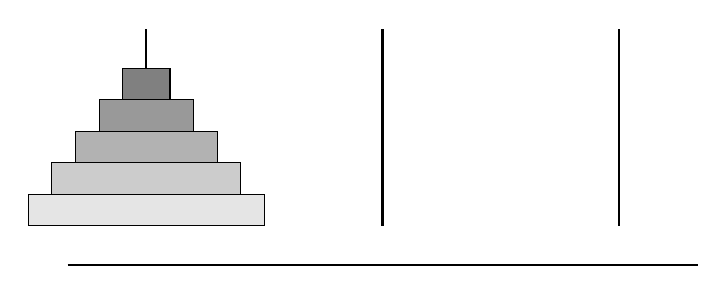
\begin{tikzpicture}
        % Draw the rods
            \draw[thick] (0,0) -- (0,2.5);
            \draw[thick] (3,0) -- (3,2.5);
            \draw[thick] (6,0) -- (6,2.5);
            
        % Draw the base
            \draw[thick] (-1,-0.5) -- (7,-0.5);
            
        % Draw the disks on the first rod
            \draw[fill=gray!20] (-1.5,0) rectangle (1.5,0.4);
            \draw[fill=gray!40] (-1.2,0.4) rectangle (1.2,0.8);
            \draw[fill=gray!60] (-0.9,0.8) rectangle (0.9,1.2);
            \draw[fill=gray!80] (-0.6,1.2) rectangle (0.6,1.6);
            \draw[fill=gray!100] (-0.3,1.6) rectangle (0.3,2);
    \end{tikzpicture}
    \caption{Illustration of the Hanoi Towers problem with disks.}
    \label{fig:hanoi}
\end{figure}

The Hanoi Towers problem consists of three rods and $n$ disks of different sizes. The disks are stacked in decreasing order of size on the first rod. The goal is to move all the disks to the third rod, following the rules:
\begin{itemize}
    \item Only one disk can be moved at a time.
    \item A disk can only be placed on top of a larger disk.
\end{itemize}

Let $h(n)$ be the number of moves required to move $n$ disks from the first to the third rod. The recurrence relation is:
\[
h(n) = 2h(n-1) + 1 = 2(2h(n-2) + 1) + 1 = 2^2 h(n-2) + 2 + 1 =
\]
\[
\dots = 2^n h(0) + 2^{n-1} + 2^{n-2} + \dots + 2^1 + 1
\]
\[
h(n) = 2^n - 1
\]

\subsection{Derangements as recurrence}
\begin{figure}[!h]
    \centering
    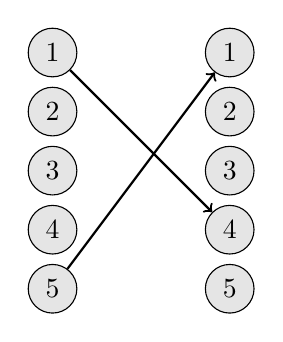
\begin{tikzpicture}[scale=1.5]
        % Nodes on the left
        \foreach \i in {1,2,3,4,5} {
            \node[circle, draw, fill=gray!20, minimum size=0.6cm] (L\i) at (0, 3-\i*0.5) {\i};
        }
        
        % Nodes on the right
        \foreach \i in {1,2,3,4,5} {
            \node[circle, draw, fill=gray!20, minimum size=0.6cm] (R\i) at (1.5, 3-\i*0.5) {\i};
        }
        
        % Arrows
        \draw[->, thick] (L1) -- (R4);
        \draw[->, thick] (L5) -- (R1);
    \end{tikzpicture}
    \label{fig:graph}
    \caption{Graph representation of a derangement.}
\end{figure}
\begin{itemize}
    \item Suppose $4 \rightarrow 1$ \quad $d(n-2)$ ways to derange the remaining elements.
    \item Suppose $4 \nrightarrow 1$ \quad $d(n-1)$ ways to derange the remaining elements.
\end{itemize}
\[
d(n) = (n-1)(d(n-1) + d(n-2))
\]

\subsection*{Example:}
Find a recurrence relation for the number of bit strings of length $n$ that do not contain two consecutive 0s. \\
Consider $n \geq 3$. Build the string from strings of length $n-1$.
\begin{itemize}
    \item If the last digit is 1, there are $d(n-1)$ ways to build the string.
    \item If the last digit is 0, the second-to-last digit must be 1. There are $d(n-2)$ ways to build the string.
\end{itemize}
\[
d(n) = d(n-1) + d(n-2) \quad \text{which is the Fibonacci sequence again!}
\]

\section{Linear Recurrence Relations}
\[
a_n = c_1 a_{n-1} + c_2 a_{n-2} + \dots + c_k a_{n-k} = \left\{a_n\right\}_{n=1}^{\infty}
\]
\[
\text{With } c_i \in \mathbb{R}, \quad c_k \neq 0 \quad \text{and} \quad k \geq 1 = \text{order of the recurrence relation}
\]

\[
1. \quad a_n = r^n, \quad r \in \mathbb{R}, \quad r \neq 0
\]
\[
r^n = c_1 r^{n-1} + c_2 r^{n-2} + \dots + c_k r^{n-k}
\]
\[
r^k - c_1 r^{k-1} - c_2 r^{k-2} - \dots - c_k = 0 \quad \rightarrow \text{Characteristic equation}
\]

\[
2. \quad \text{Superposition principle: the sum of solutions is also a solution} 
\]
\[
\{s_n\}, \{t_n\} \text{ are solutions } \rightarrow \{s_n + t_n\} \text{ is also a solution}
\]

\[
s_n = c_1 s_{n-1} + c_2 s_{n-2} + \dots + c_k s_{n-k}
\]
\[
t_n = c_1 t_{n-1} + c_2 t_{n-2} + \dots + c_k t_{n-k}
\]
\[
s_n + t_n = c_1 (s_{n-1} + t_{n-1}) + c_2 (s_{n-2} + t_{n-2}) + \dots + c_k (s_{n-k} + t_{n-k})
\]

\subsection{The $k = 2$ case}
\[
a_n = c_1 a_{n-1} + c_2 a_{n-2}, \quad c_2 \neq 0
\]
\[
a_0 = \alpha_0, \quad a_1 = \alpha_1, \quad \text{initial conditions}
\]

\[
\text{Then, } \quad r^2 - c_1 r - c_2 = 0
\implies \text{solutions } r_1 \neq r_2
\]

General solution:
\[
a_n = \beta_1 r_1^n + \beta_2 r_2^n
\]

Use the initial conditions to find $\beta_1$ and $\beta_2$.
\[
a_0 = \beta_1 + \beta_2 = \alpha_0 \quad \rightarrow \beta_2 = \alpha_0 - \beta_1
\]
\[
a_1 = \beta_1 r_1 + \beta_2 r_2 = \alpha_1 \quad \rightarrow \alpha_1 = \beta_1 r_1 + (\alpha_0 - \beta_1) r_2
\]

\[
\alpha_1 - \alpha_0 r_2 = \beta_1 (r_1 - r_2) \quad \rightarrow \beta_1 = \frac{\alpha_1 - \alpha_0 r_2}{r_1 - r_2}
\]

\[
\text{Then, } \quad \beta_2 = \alpha_0 - \frac{\alpha_1 - \alpha_0 r_2}{r_1 - r_2} = \frac{\alpha_0 r_1 - \alpha_1}{r_1 - r_2}
\]

\subsection*{Example:}
\[
a_n = a_{n-1} + 2a_{n-2}, \quad a_0 = 2, \quad a_1 = 7
\]
\[
r^2 - r - 2 = 0 \quad \rightarrow r_1 = 2, \quad r_2 = -1
\]
\[
a_n = \beta_1 2^n + \beta_2 (-1)^n
\]

\[
2 = \beta_1 + \beta_2 \quad \rightarrow \beta_2 = 2 - \beta_1
\]
\[
7 = 2 \beta_1 - \beta_2 \quad \rightarrow 7 = 2 \beta_1 - (2 - \beta_1) \quad \rightarrow \beta_1 = 3
\]
\[
\text{Then, } \quad \beta_2 = 2 - 3 = -1
\]

\[
a_n = 3 \cdot 2^n - (-1)^n
\]

\subsection*{Example: Fibonacci sequence}
\[
F_n = F_{n-1} + F_{n-2}, \quad F_0 = 0, \quad F_1 = 1
\]
\[
r^2 - r - 1 = 0 \quad \rightarrow r_1 = \frac{1 + \sqrt{5}}{2}, \quad r_2 = \frac{1 - \sqrt{5}}{2}
\]

\[
0 = \beta_1 + \beta_2 \quad \rightarrow \beta_2 = -\beta_1
\]
\[
1 = \beta_1 \frac{1 + \sqrt{5}}{2} - \beta_1 \frac{1 - \sqrt{5}}{2} \quad \rightarrow \beta_1 = \frac{1}{\sqrt{5}}
\]

\[
F_n = \frac{1}{\sqrt{5}} \left( \left( \frac{1 + \sqrt{5}}{2} \right)^n - \left( \frac{1 - \sqrt{5}}{2} \right)^n \right)
\]

\subsection*{Special case: $r_1 = r_2$}
\[
r^2 - c_1 r - c_2 = 0 \quad \rightarrow \text{With } r_1 = r_2 = r
\]
\[
\text{Then, the general solution is } a_n = \beta_1 r^n + \beta_2 n r^n
\]

\[
a_0 = \beta_1 = \alpha_0 \quad \rightarrow \beta_1 = \alpha_0
\]
\[
a_1 = \beta_1 r + \beta_2 r = \alpha_1 \quad \rightarrow \beta_2 = \frac{\alpha_1 - \alpha_0 r}{r}
\]

\subsection*{Example:}
\[
a_n = 6 a_{n-1} - 9 a_{n-2}, \quad a_0 = 1, \quad a_1 = 6
\]
\[
r^2 - 6r + 9 = 0 \quad \rightarrow r = 3
\]

\[
a_n = \beta_1 3^n + \beta_2 n 3^n
\]
\[
1 = \beta_1 \quad \rightarrow \beta_1 = 1
\]
\[
6 = 3 \beta_1 + 3 \beta_2 \quad \rightarrow 6 = 3 + 3 \beta_2 \quad \rightarrow \beta_2 = 1
\]

\[
a_n = 3^n + n 3^n
\]

\subsection{Theorem: Solution of degree $k$ recurrence relations with constant coefficients}
Let $a_n = c_1 a_{n-1} + c_2 a_{n-2} + \dots + c_k a_{n-k}, \quad c_i \in \mathbb{R}, \quad c_k \neq 0$ be a linear recurrence relation with constant coefficients.
Consider the characteristic equation:
\[
r^k - c_1 r^{k-1} - c_2 r^{k-2} - \dots - c_k = 0
\]
Assume it has different roots $r_1, r_2, \dots, r_t$, with multiplicities $m_1, m_2, \dots, m_t$, with $m_1 + m_2 + \dots + m_t = k$.
Then, the general solution is:

\[
a_n = (\beta_{10} + \beta_{11} n + \beta_{12} n^2 + \dots + \beta_{1m_1} n^{m_1-1}) r_1^n + \dots + (\beta_{t0} + \beta_{t1} n + \beta_{t2} n^2 + \dots + \beta_{tm_t} n^{m_t-1}) r_t^n
\]
\[
a_n = \sum_{i=1}^{t} \sum_{j=1}^{m_i} \beta_{ij} n^{j-1} r_i^n
\]

Given $k$ initial conditions $a_0 = \alpha_0, a_1 = \alpha_1, \dots, a_{k-1} = \alpha_{k-1}$, the coefficients $\beta_{ij}$ can be found by solving the system of linear equations.

\subsection*{Example:}
\[
a_n = -3 a_{n-1} - 3 a_{n-2} - a_{n-3}, \quad a_0 = 1, \quad a_1 = -2, \quad a_2 = -1
\]
\[
r^3 + 3r^2 + 3r + 1 = 0 \quad \rightarrow r = -1, \text{ with multiplicity } 3
\]

\[
a_n = (\beta_1 + \beta_2 n + \beta_3 n^2) (-1)^n
\]
\[
1 = \beta_1 \quad \rightarrow \beta_1 = 1
\]
\[
-2 = (1 + 2 \beta_2 + \beta_3) (-1) \quad \rightarrow 1 = \beta_2 + \beta_3 \quad \rightarrow \beta_2 = 3
\]
\[
-1 = (1 + 2 \beta_2 + 4 \beta_3) \quad \rightarrow -1 = 1 + 2 \beta_2 + 4 \beta_3 \quad \rightarrow \beta_3 = -2
\]

\[
a_n = 1 + 3n - 2n^2 (-1)^n
\]

\subsection{Nonhomogeneous Recurrence Relations}
\[
a_n = c_1 a_{n-1} + c_2 a_{n-2} + \dots + c_k a_{n-k} + F(n)
\]
\[
\text{With } F(n) \text{ a function of } n
\]

\paragraph{Theorem:}
The general solution of the nonhomogeneous case is:
\[
a_n = a_n^{(h)} + a_n^{(p)}
\]

Where $a_n^{(h)}$ is the general solution of the homogeneous case, with $F(n) = 0$, and $a_n^{(p)}$ is a particular solution of the nonhomogeneous case.

\subsection*{Example:}
\[
a_n = 3 a_{n-1} + 2 a_{n-2} + 2^n, \quad a_1 = 3
\]
\[
\text{Homogeneous: } \quad r - 3 = 0 \quad \rightarrow r = 3
\]
\[
\text{General solution: } \quad a_n^{(h)} = \beta 3^n
\]

\[
\text{Particular solution: assume } p_n = cn + d
\]
\[
cn + d = 3(c(n-1) + d) + 2n
\]
\[
cn + d = 3cn - 3c + 3d + 2n
\]
\[
c = 3c + 2 \implies c = -1
\]
\[
d = 3c + 3d \implies d = \frac{-3}{2}
\]

\[
\text{Particular solution: } \quad p_n = -n - \frac{3}{2}
\]
\[
\text{General solution: } \quad a_n = \beta 3^n - n - \frac{3}{2}
\]

\[
a_1 = 3 = \beta 3 - 1 - \frac{3}{2} 
\]
\[
3 \beta = \frac{11}{2} \implies \beta = \frac{11}{6}
\]

\[
a_n = \frac{11}{6} 3^n - n - \frac{3}{2}
\]

\subsection*{Example:}
\[
a_n = 5 a_{n-1} - 6 a_{n-2} + 7^n
\]
\[
r^2 - 5r + 6 = 0 \quad \rightarrow r = 2, 3
\]

\[
a_n^{(h)} = \beta_1 3^n + \beta_2 2^n
\]

\[
p_n = c 7^n = 5(c 7^{n-1}) - 6(c 7^{n-2}) + 7^n
\]
\[
49c = 35c - 6c + 49 \quad \rightarrow 20c = 49 \quad \rightarrow c = \frac{49}{20}
\]

\[
a_n = \beta_1 3^n + \beta_2 2^n + \frac{49}{20} 7^n
\]
\[
a_0 = 1, \quad a_1 = 2
\]

\[
1 = \beta_1 + \beta_2 + \frac{49}{20} \quad \rightarrow \beta_1 + \beta_2 = -\frac{29}{20}
\]
\[
2 = 3 \beta_1 + 2 \beta_2 + \frac{49}{20} \quad \rightarrow 3 \beta_1 + 2 \beta_2 = -\frac{11}{20}
\]
\[
\beta_1 = -\frac{9}{20}, \quad \beta_2 = -\frac{1}{4}
\]

\[
a_n = -\frac{9}{20} 3^n - \frac{1}{4} 2^n + \frac{49}{20} 7^n
\]

\subsection{Theorem: Particular solutions}
Let $a_n = c_1 a_{n-1} + c_2 a_{n-2} + \dots + c_k a_{n-k} + F(n)$ be a linear recurrence relation with constant coefficients and $F(n) = (b_t n^t + b_{t-1} n^{t-1} + \dots + b_1 n + b_0) s^n$.
Then, a particular solution if $s$ is not a root is:
\[
p_n = (d_t n^t + d_{t-1} n^{t-1} + \dots + d_1 n + d_0) s^n
\]

If $s$ is a root of the characteristic equation with multiplicity $m$, then the particular solution is:
\[
p_n = (d_t n^t + d_{t-1} n^{t-1} + \dots + d_1 n + d_0) s^n n^m
\]

\subsection*{Example:}
\[
a_n = 6 a_{n-1} - 9 a_{n-2} + F(n)
\]
\[
F(n) = 3^n, \quad F(n) = n 3^n, \quad F(n) = n^2 2^n, \quad F(n) = (1 + n) 2^n
\]

\[
r^2 - 6r + 9 = 0 \quad \rightarrow r = 3 \text{ with multiplicity } 2
\]

For $F(n) = 3^n$:
\[
p_n = d n^2 3^n
\]

For $F(n) = n 3^n$:
\[
p_n = n^2 (d_1 n + d_0) \cdot 3^n
\]

For $F(n) = n^2 2^n$:
\[
p_n = (d_2 n^2 + d_1 n + d_0) 2^n
\]

For $F(n) = (1 + n) 2^n$:
\[
p_n = n^2 (d_2 n^2 d_1 n + d_0) 3^n
\]

\subsection{The $r = 1$ case}
\[
F(n) = (b_t n^t + b_{t-1} n^{t-1} + \dots + b_1 n + b_0) \cdot 1^n, \quad \text{with } r = 1 \text{ a root}
\]

\subsection*{Example:}
\[
a_n = \sum_{k = 1}^{n} k
\]
\[
a_n = a_{n-1} + n, \quad a_1 = 1
\]
\[
r - 1 = 0 \quad \rightarrow r = 1, \quad x_h = c 1^n = c
\]
\[
x_p = (p_1 n + p_0) \cdot n = p_1 n^2 + p_0 n
\]

\[
p_1 n^2 + p_0 n = p_1 (n-1)^2 + p_0 (n-1) + n
\]
\[
p_1 n^2 + p_0 n = p_1 n^2 - 2 p_1 n + p_1 + p_0 n - p_0 + n
\]
\[
0n + 0 = (1 - 2p_1) n + (p_1 - p_0)
\]

\[
p_1 = \frac{1}{2}, \quad p_0 = \frac{1}{2}
\]
\[
\implies a_n = c + \frac{n^2}{2} + \frac{n}{2}, \quad a_1 = 1 \implies c = 0
\]
\[
a_n = \frac{n^2 + n}{2} = \frac{n(n+1)}{2}
\]

\section{Generating Functions}
The generating function for a sequence $\{a_0, a_1, a_2, \dots\}$ of real numbers is the infinite formal series:
\[
G(x) = a_0 + a_1 x + a_2 x^2 + \dots a_k x^k = \sum_{k=0}^{\infty} a_k x^k
\]

\subsection*{Example:}
\[
a_k = k + 1 \quad \rightarrow \quad G(x) = 1 + 2x + 3x^2 + 4x^3 + \dots = \sum_{k=0}^{\infty} (k+1) x^k
\]

\[
a_k = 2^k \quad \rightarrow \quad G(x) = 1 + 2x + 4x^2 + 8x^3 + \dots = \sum_{k=0}^{\infty} 2^k x^k
\]

\subsection{Finite sequence}
\[
\{a_0, a_1, a_2, \dots, a_k\} \quad \rightarrow \quad G(x) = a_0 + a_1 x + a_2 x^2 + \dots + a_k x^k
\]

Which is like $a_i = 0$ for $i \geq k + 1$.

\subsection*{Example:}
\[
\{1, 1, 1, 1, 1, 1\} \quad \rightarrow \quad G(x) = 1 + x + x^2 + x^3 + x^4 + x^5 = \frac{x^6 - 1}{x - 1}
\]

\subsection*{Example:}
\[
a_k = \binom{n}{k} \quad \rightarrow \quad G(x) = (1 + x)^n = \sum_{k=0}^{n} \binom{n}{k} x^k
\]

\subsection{Frequent and important generating functions}

\begin{enumerate}
    \item $$\frac{1}{1 - x} = 1 + x + x^2 + x^3 + \dots = \sum_{k=0}^{\infty} x^k, \text{converges for } |x| < 1$$
          $$\frac{1}{1 - ax} = 1 + ax + a^2 x^2 + a^3 x^3 + \dots = \sum_{k=0}^{\infty} a^k x^k, \text{converges for } |x| < \frac{1}{|a|}$$
    \item $$\begin{cases}
                G_1(x) = \sum_{k = 0}^{\infty} a_kx^k \\
                G_2(x) = \sum_{k = 0}^{\infty} b_kx^k
            \end{cases} \implies 
            \begin{cases}
                G_1(x) + G_2(x) = \sum_{k = 0}^{\infty} (a_k + b_k)x^k \\
                G_1(x) \cdot G_2(x) = \sum_{k = 0}^{\infty} \left( \sum_{i = 0}^{k} a_i b_{k-i} \right)x^k
            \end{cases}$$
    \item $$\frac{1}{(1 - x)^2} = 1 + 2x + 3x^2 + 4x^3 + \dots = \frac{1}{1 - x} \cdot \frac{1}{1 - x} = \sum_{k = 0}^{\infty} x^k \cdot \sum_{j = 0}^{\infty} x^j = \sum_{k = 0}^{\infty} (k + 1)x^k$$
    \item $$\frac{1}{(1 - x)^2} = \frac{d}{dx} \left( \frac{1}{1 - x} \right) = \frac{d}{dx} \left( \sum_{k = 0}^{\infty} x^k \right) = \sum_{k = 0}^{\infty} kx^{k-1} = \sum_{k = 0}^{\infty} (k + 1)x^k$$
    \item $$\textbf{Definition:} \quad \binom{u}{k} = 
            \begin{cases}
                \dfrac{u(u-1)\dots(u-k+1)}{k!} & \text{if } k > 0 \\
                1 & \text{if } k = 0
            \end{cases}
            \quad \text{for } u \in \mathbb{R} \text{ and } k \in \mathbb{N}$$
            $$\text{If } u = -3 \text{ and } k = 2 \text{ then } \binom{-3}{2} = \frac{-3 \cdot -4}{2} = 6$$
            $$\text{If } u = \frac{1}{2} \text{ and } k = 3 \text{ then } \binom{\frac{1}{2}}{3} = \dfrac{\dfrac{1}{2} \cdot \dfrac{-1}{2} \cdot \dfrac{-3}{2}}{6} = \frac{1}{16}$$
            
            $$\textbf{Special case: } u \text{ is a negative integer } u = - n, \quad n \in \mathbb{N}$$
            $$\binom{-n}{r} = \frac{(-n)(-n-1)\dots(-n-r+1)}{r!} = \frac{(-1)^r n(n+1)\dots(n+r-1)}{r!} = $$
            $$= (-1)^r \binom{n+k-1}{k} = (-1)^r CR_n^r$$
            
            $$\textbf{Extended Binomial Theorem:} \quad (1 + x)^u = \sum_{k = 0}^{\infty} \binom{u}{k} x^k$$

            $$\textbf{Special case: } u = -n \text{ and } n \in \mathbb{N} $$
            $$(1 + x)^{-n} = \sum_{k = 0}^{\infty} \binom{-n}{k} x^k = \sum_{k = 0}^{\infty} (-1)^k \binom{n + k - 1}{k} x^k$$
            $$(1 - x)^{-n} = \sum_{k = 0}^{\infty} \binom{n + k - 1}{k} x^k$$ 
\end{enumerate}

\subsection{Applications of generating functions}
\subsection*{Example:}
Find the number of integer solutions of $x_1 + x_2 + x_3 = 17$ when $2 \leq x_1 \leq 5$, $3 \leq x_2 \leq 6$, and $3 \leq x_4 \leq 7$.
\[
G(x) = (x^2 + x^3 + x^4 + x^5)(x^3 + x^4 + x^5 + x^6)(x^4 + x^5 + x^6 + x^7) =
\]
We look for the coefficient of $x^{17}$ in $G(x)$.
\[
x^5 \cdot x^5 \cdot x^7 + x^5 \cdot x^6 \cdot x^6 + x^4 \cdot x^6 \cdot x^7 \rightarrow 3 \text{ solutions}
\]

\subsection*{Example:}
In how many ways can we distribute 8 identical cookies among 3 children so that each child recieves at least 2 and and no more than 4 cookies?
\[
G(x) = (x^2 + x^3 + x^4)^3 = x^6 (1 + x + x^2)^3 = x^6 (1 + 3x + 3x^2 + x^3) = x^6 + 3x^7 + 3x^8 + x^9
\]
\[
\text{Coefficient of } x^8 = 3 \text{ ways}
\]

\subsection*{Example:}
In how many ways can we gather $r$ euros using coins of 1 and 2 and notes of 5?
\[
G(x) = (1 + x + x^2 + \dots)(1 + x^2 + x^4 + \dots)(1 + x^5 + x^{10} + \dots) 
\]
For $r = 7$:
\[
(1 + x + x^2 + x^3 + x^4 + x^5 + x^6 + x^7)(1 + x^2 + x^4 + x^6)(1 + x^5) =
\]
\[
x^7 \cdot 1 \cdot 1 + x \cdot x^6 \cdot 1 + x^5 \cdot x^2 \cdot 1 + x^3 \cdot x^4 \cdot 1 + x^2 \cdot x^5 \cdot 1 + x^4 \cdot x^3 \cdot 1 + x^6 \cdot x^2 \cdot 1 = 6 \text{ ways}
\]

Same, but now order matters:

To insert $n$ coins or notes adding up to $r$ euros:
\[
(x + x^2 + x^5)^n, \quad \text{coefficient of } x^r
\]
\[
G(x) = 1 + (x + x^2 + x^5) + (x + x^2 + x^5)^2 + \dots = \frac{1}{1 - (x + x^2 + x^5)}
\]

\subsection*{Example:}
Suppose we have 3 green balls, 3 blue balls, 2 red balls and 1 white ball. How many ways are there to choose four of them?
\[
x_g + x_b + x_r + x_w = 4
\]
\[
G(x) = (1 + x + x^2 + x^3)(1 + x + x^2 + x^3)(1 + x + x^2) (1 + x) = (1 + x + x^2 + x^3)^2 (1 + x + x^2) (1 + x)
\]
\[
G(x) = \frac{1 - x^4}{1 - x} \cdot \frac{1 - x^4}{1 - x} \cdot \frac{1 - x^3}{1 - x} \cdot \frac{1 - x^2}{1 - x} = \frac{(1 - x^4)^2 (1 - x^3) (1 - x^2)}{(1 - x)^4} = 
\]
\[
= (1 - 2x^4)(1 - x^3)(1 - x^2) = (1 - x^2 - x^3 - 2x^4 + \dots)(1 + 4x + \binom{5}{2}x^2 + \binom{6}{3}x^3 + \binom{7}{4}x^4 + \dots) =
\]
\[
\binom{7}{4} - \binom{5}{2} - 4 - 2 = 19
\]
\[
\frac{1}{(1 - x)^4} = \sum_{n = 0}^{\infty} \binom{n + 3}{3} x^n = \binom{7}{4}
\]

\subsection*{Example:}
18 candies in 5 boxes with none empty, an even number of candies in each box, with no more than 10 candies in thee first two and 2 to 6 candies in the last three.
\[
G(x) = (x^2 + x^4 + x^6 + x^8 + x^{10})^2(x^2 + x^4 + x^6)^3 =
\]
\[
= x^4 (1 + x^2 + x^4 + x^6 + x^8)^2 x^6(1 + x^2 + x^4)^3 = x^{10} \frac{(1 - x^{10})^2}{(1 - x^2)^2} \frac{(1 - x^6)^3}{(1 - x^2)^3} = x^{10} \frac{(1 - x^{10})^2 (1 - x^6)^3}{(1 - x^2)^5}
\]
\[
\text{Coefficient of } x^{8}: \quad (1 - x^{10})^2 (1 - x^6)^3 \rightarrow (1 - 3x^6 + 3x^{12} - x^{18}) \rightarrow (1 - 3x^6)
\]
\[
\frac{1}{(1 - x^2)^5} = \sum_{n = 0}^{\infty} \binom{n + 4}{n} x^{2n}
\]
\[
(1 - 3x^6)\left(1 + 5x^2 + \binom{6}{2}x^4 + \binom{7}{3}x^6 + \binom{8}{4}x^8 + \dots\right) \rightarrow -15 + \binom{8}{4} = 55
\]

\subsection{Recurrence relations and generating functions}
\subsection*{Example:}
\[
a_k = 3a_{k-1}, \quad a_0 = 2
\]
\[
r = 3 \rightarrow a_k = c3^k \rightarrow a_k = 2 \cdot 3^k
\]

Now with:
\[
G(x) = \sum_{k = 0}^{\infty} a_k x^k 
\]
\[
G(x) - 3xG(x) = \sum_{k = 0}^{\infty} a_k x^k - 3 \sum_{k = 1}^{\infty} a_{k-1} x^k = a_0 + \sum_{k = 1}^{\infty} a_k x^k - 3 \sum_{k = 1}^{\infty} a_{k-1} x^k =
\]
\[
= 2 + \sum_{k = 1}^{\infty} (a_k - 3a_{k-1}) x^k = 2, \quad \text{since } a_k = 3a_{k-1}
\]
\[
G(x) = \frac{2}{1 - 3x} = 2 \sum_{k = 0}^{\infty} 3^k x^k \rightarrow a_k = 2 \cdot 3^k
\]

\subsection*{Example:}
\[
a_n = 8a_{n-1} + 10^{n-1}, \quad a_1 = 9, \quad n \geq 0
\]
\[
G(x) = \sum_{n = 1}^{\infty} a_n x^n
\]

Introduction of $a_0$: $a_1 = 8a_0 + 10^0 = 9 \rightarrow a_0 = 1$
\[
a_n x^n = 8a_{n-1} x^n + 10^{n-1} x^n
\]
\[
\sum_{n = 1}^{\infty} a_n x^n = 8 \sum_{n = 1}^{\infty} a_{n-1} x^{n} + \sum_{n = 1}^{\infty} 10^{n-1} x^n 
\]
\[
G(x) - a_0 = 8x \sum_{n = 1}^{\infty} a_{n-1} x^{n - 1} + x \sum_{n = 1}^{\infty} 10^{n-1} x^ {n-1} = 
\]
\[
= 8x \sum_{n = 0}^{\infty} a_n x^n + x \sum_{n = 0}^{\infty} 10^n x^n = 8xG(x) + \frac{x}{1 - 10x}
\]
\[ 
G(x) - a_0 = 8xG(x) + \frac{x}{1 - 10x} = \frac{1 - 9x}{1 - 10x}
\]
\[
G(x) = \frac{1 - 9x}{(1 - 10x)(1 - 8x)} 
\]
\[
G(x) = \frac{A}{1 - 8x} + \frac{B}{1 - 10x} = \frac{1}{2} \left( \frac{1}{1 - 8x} + \frac{1}{1 - 10x} \right) = 
\]
\[
= \frac{1}{2} \left( \sum_{n = 0}^{\infty} 8^n x^n + \sum_{n = 0}^{\infty} 10^n x^n \right) \rightarrow a_n = \frac{1}{2} (8^n + 10^n)
\]
Where $A = \frac{1}{2}$ and $B = \frac{1}{2}$, since
\[
1 - 9x = A(1 - 10x) + B(1 - 8x) \rightarrow 1 = A + B, \quad -9 = -10A - 8B
\]
\[
9 = 10A + 8 - 8A \rightarrow 1 = 2A \rightarrow A = \frac{1}{2}, \quad B = \frac{1}{2}
\]

\[
\textbf{Homogeneous: } r = 8 \rightarrow a_n^h = c8^n
\]
\[
a_p = D \cdot 10^n \rightarrow 10D = 8D + 1 \rightarrow D = \frac{1}{2}
\]
\[
a_n = c8^n + \frac{1}{2} \cdot 10^n
\]
\[
a_1 = 9 = c8 + 5 \rightarrow c = \frac{1}{2}
\]

\subsection*{Example:}
\[
a_n = 3a_{n-1} + n, \quad a_0 = 1, \quad n \geq 1
\]
\[
G(x) = \sum_{n = 0}^{\infty} a_n x^n
\]
\[
a_n x^n = 3a_{n-1} x^n + nx^n
\]
\[
\sum_{n = 1}^{\infty} a_n x^n = \sum_{n = 1}^{\infty} 3a_{n-1} x^n + \sum_{n = 1}^{\infty} nx^n
\]
\[
G(x) - a_0 = 3x \sum_{n = 1}^{\infty} a_{n-1} x^{n-1} + x \sum_{n = 1}^{\infty} nx^{n-1} = 3x \sum_{n = 0}^{\infty} a_n x^n + x \sum_{n = 0}^{\infty} nx^n
\]
\[
G(x) - 1 = 3xG(x) + x \sum_{n = 0}^{\infty} nx^n = 3xG(x) + x \frac{d}{dx} \left( \sum_{n = 0}^{\infty} x^n \right) = 3xG(x) + x \frac{d}{dx} \left( \frac{1}{1 - x} \right)
\]
\[
G(x) - 1 = 3xG(x) + x \frac{1}{(1 - x)^2} = 3xG(x) + \frac{x}{(1 - x)^2}
\]
\[
G(x) = \frac{1}{1 - 3x} + \frac{x}{(1 - x)^2(1 - 3x)} = \frac{A}{1 - x} + \frac{B}{(1 - x)^2} + \frac{C}{1 - 3x}
\]
\[
x = A(1 - x)(1 - 3x) + B(1 - 3x) + C(1 - x)^2 
\]

\[
\begin{cases}
    1 = B(1 - 3) \rightarrow B = -\frac{1}{2} \\
    \frac{1}{3} = C \frac{4}{9} \rightarrow C = \frac{3}{4} \\
    0 = A + B + C \rightarrow A = -\frac{1}{4}
\end{cases}
\]

\[
G(x) = \frac{7}{4} \frac{1}{1 - 3x} - \frac{1}{2} \frac{1}{(1 - x)^2} - \frac{1}{4} \frac{1}{1 - x}
\]
\[
G(x) = \sum_{n = 0}^{\infty} \left( \frac{7}{4} 3^n - \frac{1}{2} (n + 1) - \frac{1}{4} \right) 
\]

\subsection*{Example:}
\[
a_{n+2} - 5a_{n+1} + 6a_n = 2, \quad x_0 = 3, \quad x_1 = 7, \quad n \geq 0
\]
\[
G(x) = \sum_{n = 0}^{\infty} a_n x^n = 3 + 7x + \sum_{n = 2}^{\infty} a_n x^n
\]
Multiply by $x^{n+2}$:
\[
a_{n+2} x^{n+2} - 5a_{n+1} x^{n+2} + 6a_n x^{n+2} = 2x^{n+2}
\]
Sum over all allowed $n$:
\[
\sum_{n = 0}^{\infty} a_{n+2} x^{n+2} - 5 \sum_{n = 0}^{\infty} a_{n+1} x^{n+2} + 6 \sum_{n = 0}^{\infty} a_n x^{n+2} = 2 \sum_{n = 0}^{\infty} x^{n+2}
\]
Match the power of $x$ with the index of $a_n$ extracting as many factors $x$ as needed:
\[
\sum_{n = 0}^{\infty} a_{n+2} x^{n+2} - 5x \sum_{n = 0}^{\infty} a_{n+1} x^{n+1} + 6x^2 \sum_{n = 0}^{\infty} a_n x^n = 2x^2 \sum_{n = 0}^{\infty} x^n
\]
Shift the index of the sums:
\[
\sum_{n = 2}^{\infty} a_n x^n - 5x \sum_{n = 1}^{\infty} a_n x^n + 6x^2 \sum_{n = 0}^{\infty} a_n x^n = 2x^2 \sum_{n = 0}^{\infty} x^n
\]
Identify functions (use initial conditions as needed):
\[
G(x) - 3 - 7x = -5x(G(x) - 3) + 6x^2 G(x) = \frac{2x^2}{1 - x}
\]
Solve for $G(x)$:
\[
G(x) (1 - 5x + 6x^2) = 3 + 7x - 15x + \frac{2x^2}{1 - x} 
\]
\[
G(x) = \frac{3 - 8x}{1 - 5x + 6x^2} + \frac{2x^2}{(1 - x)(1 - 5x + 6x^2)}
\]
\[
G(x) = \frac{3 - 8x}{(1 - 2x)(1 - 3x)} + \frac{2x^2}{(1 - x)(1 - 2x)(1 - 3x)}
\]
\[
G(x) = \frac{2}{1 - 3x} + \frac{1}{1 - x} = 2 \sum_{n = 0}^{\infty} 3^n x^n + \sum_{n = 0}^{\infty} x^n
\]
\[
a_n = 2 \cdot 3^n + 1
\]

\subsection*{Example:}
A person has 6 friends: $\{A, B, C, D, E, F\}$. He wants to invite 4 of them home, but A and B cannot come together, and neihter can E and F, because of personal conflicts. If the invitation is made at random, what is the possibiliy that the dinner goes well?
\[
P = \frac{\text{number of good outcomes}}{\text{total number of groups of 4 friends}}
\]

\[
\text{Total number of groups of 4 friends: } \binom{6}{4} = 15
\]

\[
S_{AB} = \text{number of groups with A and B together} = \binom{4}{2} = 6
\]
\[
S_{EF} = \text{number of groups with E and F together} = \binom{4}{2} = 6
\]
\[
S_{ABEF} = \text{number of groups with A and B and E and F together} = \binom{2}{2} = 1
\]

\[
\text{Number of good outcomes: } 15 - 6 - 6 + 1 = 4
\]
\[
P = \frac{4}{15}
\]

\subsection*{Example:}
In how many ways can we order the letters A, E, M, O, Y, U in 6-letter strings without letter repetition that do not contain the word "ME" or "YOU"?
\[
\text{Total number of strings: } 6! = 720
\]

\[
S_{ME} = \text{number of strings with "ME"} = 5! = 120
\]
\[
S_{YOU} = \text{number of strings with "YOU"} = 4! = 24
\]
\[
S_{MEYOU} = \text{number of strings with "ME" and "YOU"} = 3! = 6
\]

\[
\text{Number of good strings: } 720 - 120 - 24 + 6 = 582
\]

\subsection*{Example:}
A message is made of 12 symbols in a specified order. To transmit it, you have to send 45 blanks along with the symbols, and every two symbols must be searated by at least 3 blank. How many different messages can be sent?
\[
CR_{11}^{12} = \binom{11 + 12 - 1}{12} = \binom{22}{12} = 646646
\]

\subsection*{Example:}
How many subsets of 4 elements can be formed from elements of $\{1, 2, 3, \dots, 13, 14, 15\}$ such that no subset contains two consecutive numbers?
\[
\text{Subsets look like: } \{n_1, n_2, n_3, n_4\} \quad 1 \leq n_i \leq 15
\]
\[
\text{For non-consecutive numbers: } \{n_1, n_2, n_3, n_4\} \quad n_2 - n_1 \geq 2, \quad n_3 - n_2 \geq 2, \quad n_4 - n_3 \geq 2
\]
\[
\begin{cases}
    x_1 = n_1 \geq 1 \\
    x_2 = n_2 - n_1 \geq 2 \\
    x_3 = n_3 - n_2 \geq 2 \\
    x_4 = n_4 - n_3 \geq 2 \\
\end{cases} \implies 
n_4 = x_4 + x_3 + x_2 + x_1 \leq 15
\]
\[
\begin{cases}
    y_1 = x_1 - 1 \geq 0 \\
    y_2 = x_2 - 2 \geq 0 \\
    y_3 = x_3 - 2 \geq 0 \\
    y_4 = x_4 - 2 \geq 0 \\
\end{cases} \implies
y_4 + y_3 + y_2 + y_1 \leq 8
\]
\[
y_1 + y_2 + y_3 + y_4 + y_5 = 8
\]

\[
CR_5^8 = \binom{8 + 5 - 1}{8} = \binom{12}{8} = 495
\]

\subsection*{Example:}
How many ways are there to choose 25 objects from 7 categories so that there are no more than 6 and no fewer than 2 objects in each category?
\[
G(x) = (x^2 + x^3 + x^4 + x^5 + x^6)^7 = x^{14} (1 + x + x^2 + x^3 + x^4)^7 = x^{14} \left( \frac{1 - x^5}{1 - x} \right)^7
\]
We need the coefficient of $x^{11}$:
\[
(1 - x^5)^7 = 1 - 7x^5 + 21x^{10} - \dots
\]
\[
\frac{1}{1 - x}^7 = \sum_{n = 0}^{\infty} \binom{n + 6}{n} x^n = \binom{6}{0} + \binom{7}{1}x + \dots + \binom{12}{6}x^6 + \dots + \binom{17}{11}x^{11} + \dots
\]
So the coefficient of $x^{11}$ is:
\[
\binom{17}{11} - 7 \binom{12}{6} + 21 \binom{7}{1} = 6055
\]

\subsection*{Example:}
\[
a_{n + 2} - 2a_{n + 1} + a_n = 2^n, \quad a_0 = 1, \quad a_1 = 2
\]
\[
\text{Homogeneous: } r^2 - 2r + 1 = 0 \rightarrow r = 1 \rightarrow a_n^h = c_1 + c_2 n
\]
\[
a_n = c_1 + c_2 n + a_n^p
\]
\[
\text{Particular: } a_{n + 2} - 2a_{n + 1} + a_n = 2^n \rightarrow a_n^p = 2^n
\]
\[
a_n = c_1 + c_2 n + 2^n
\]
\[
a_0 = 1 = c_1 + 2^0 \rightarrow c_1 = 0
\]
\[
a_1 = 2 = c_2 + 2^1 \rightarrow c_2 = 0
\]
\[
a_n = 2^n
\]

\subsection*{Example:}
Given the recurrence relation:
\[
a_{n+2} = 2a_{n+1} + a_n = 2^n, \quad a_0 = 1, \quad a_1 = 2
\]

Multiplying both sides by \( x^n \) and summing over all \( n \):
\[
\sum_{n=0}^{\infty} a_{n+2} x^n = 2 \sum_{n=0}^{\infty} a_{n+1} x^n + \sum_{n=0}^{\infty} a_n x^n + \sum_{n=0}^{\infty} 2^n x^n
\]

Defining the generating function:
\[
G(x) = \sum_{n=0}^{\infty} a_n x^n
\]

We rewrite the summations:
\[
\sum_{n=0}^{\infty} a_{n+2} x^n = G(x) - a_0 - a_1 x
\]
\[
\sum_{n=0}^{\infty} a_{n+1} x^n = x \sum_{n=1}^{\infty} a_n x^{n-1} = x(G(x) - a_0)
\]

Using these, we derive:
\[
G(x) - 1 - 2x - 2x(G(x) - 1) + x^2 G(x) = x^2 \sum_{n=0}^{\infty} 2^n x^n = \frac{x^2}{1-2x}
\]
\[
G(x) \left[1 - 2x + x^2 \right] - 1 = \frac{x^2}{1-2x}
\]
\[
G(x) = \frac{1}{(1-x)^2} + \frac{x^2}{(1-2x)(1-x)^2} = \frac{1}{1-2x}
\]

Since:
\[
\frac{1}{1-2x} = \sum_{n=0}^{\infty} (2x)^n
\]

we conclude:
\[
a_n = 2^n
\]

\subsection*{Example:}
\begin{enumerate}
    \item How many words can be formed with at most 5 letters of WATER?
    \item How many of them do not contain W?
    \item How many of them contain neither W nor E?
    \item How many of them contain both W and E?
\end{enumerate}

For (i)
\[
P_5 + V(5,1) + V(5,3) + V(5,2) + V(5,1)
\]
\[
\frac{5!}{0!} + \frac{5!}{4!} + \frac{5!}{2!} + \frac{5!}{3!} + \frac{5!}{4!}
\]

For (ii):
\[
V(4,1) + V(4,2) + V(4,3) + P_4
\]

For (iii):
\[
V_3^1 + V_3^2 + P_3
\]

For (iv):
\[
P_2 + 3 P_3 + \binom{3}{2} P_4 + P_5
\]

\subsection*{Example:}
A soccer team has 3 Goalkeepers, 8 Defenders, 6 Midfielders, and 4 Forwards. The coach wants to pick up a team with 1 Goalkeeper, 5 Defenders, 3 Midfielders, and 2 Forwards. However, he does not want players M and A to play together. 

\vspace{0.5cm}
Total Teams:
\[
\binom{3}{1} \binom{8}{5} \binom{6}{3} \binom{4}{2}
\]

Forbidden Teams:
\[
\binom{3}{1} \binom{8}{5} \binom{5}{2} \binom{3}{1}
\]

Also Consider:
\[
\binom{5}{2} \binom{3}{2} \quad \text{(with A, not B)}
\]
\[
\binom{5}{3} \binom{3}{1} \quad \text{(with B, not A)}
\]
\[
\binom{5}{3} \binom{3}{2} \quad \text{(neither)}
\]

\subsection*{Example:}

Show that in any set of 9 natural numbers, none of which has a prime factor larger than 5, there must be two whose product is a perfect square.

We express a number \( n \) in terms of its prime factorization:
\[
n = 2^x 3^y 5^z
\]

Thus, allowed numbers can be characterized by the tuple \( (x, y, z) \mod 2 \).

If we have two numbers:
\[
n = 2^{x_1} 3^{y_1} 5^{z_1}, \quad m = 2^{x_2} 3^{y_2} 5^{z_2}
\]

Then their product:
\[
n \cdot m = 2^{x_1 + x_2} 3^{y_1 + y_2} 5^{z_1 + z_2}
\]

must be a perfect square, meaning \( x_1 + x_2 \), \( y_1 + y_2 \), and \( z_1 + z_2 \) must be even.
\[
\begin{cases}
x_1 + x_2 \equiv 0 \mod 2 \\
y_1 + y_2 \equiv 0 \mod 2 \\
z_1 + z_2 \equiv 0 \mod 2
\end{cases}
\]

Since \( x, y, z \) can each take values in \( \{0,1\} \), there are \( 2^3 = 8 \) possible different tuples \( (x, y, z) \mod 2 \). By the pigeonhole principle, in any set of 9 numbers, at least two must share the same tuple, ensuring their product is a perfect square.

\subsection*{Example:}
We want to make perfumes and we have 5 ingredients: 

\textit{Vanilla, Lavender, Orange, Wood, Grass}.

\begin{enumerate}
    \item How many of them do not contain Vanilla?
    \item How many do not contain Vanilla or Wood?
    \item How many of them contain both Vanilla and Wood?
    \item How many perfumes can we make with up to 5 essences?
\end{enumerate}

The number of perfumes with up to 5 ingredients is given by 1 less than the solutions of 
\[
n_v + n_l + n_o + n_w + n_g + v \leq 5
\]
\[
n_v + n_l + n_o + n_w + n_g + v = 5
\]
\[
CR(6, 5) - 1 = 251
\]

(i)
\[
1 \leq n_l + n_o + n_w + n_g \leq 5
\]
\[
CR(5, 5) - 1 = 125
\]

(ii)
\[
1 \leq n_l + n_o + n_g \leq 5
\]
\[
CR(4, 5) - 1 = 55
\]

(iii)
\[
251 - 125 - 125 + 55 = 56
\]

\subsection*{Example:}
How many ways are there to order \( w \) white balls and \( b \) black balls in a row such that there are exactly \( k+1 \) groups of black balls?

Using combinatorial grouping:
\[ CR_{k+1}^{b-(k+1)} = \binom{b-1}{b-k-1} \]
White balls separate groups, so:
\[ \binom{w+1}{w-k} \]

\section{Correspondences}
Correspondences are relationships between elements of two sets $A$ and $B$.

For example, let:
\[
A := \{\text{cities of the world}\}, \quad B := \{\text{countries of the world}\}
\]
\[
x \in A, \quad y \in B, \quad xRy \Longleftrightarrow x \text{ is the capital of } y
\]

$H(x,y)$ means that $x$ is something with respect to $y$.
\[
\textbf{Defining set: } \quad \{x \in U \mid H(x,y)\}
\]

\subsection{Definition}
Given two sets $A$ and $B$, a correspondence of relation between $A$ and $B$ is a subset $R$ of $A \times B$, defined as:
\[
R := \{(a,b) \in A \times B \mid H(a,b)\}
\]

\subsection*{Example:}
\[
A := \{1, 2, 3, 4, 5, 6\}, \quad R := \{(m,n) \in A \times A \mid m \text{ divides } n\}
\]
\[
(1,3) \in R, \quad (2,4) \in R, \quad (3,5) \notin R
\]

\subsection*{Example:}
\[
f(x) : \mathbb{R} \rightarrow \mathbb{R}^+, \quad x \rightarrow x^2
\]
\[
f := \{(x,y) \in \mathbb{R} \times \mathbb{R}^+ \mid y = x^2\}
\]

\subsection{Representation of correspondences}
\begin{enumerate}
    \item \textbf{Arrow diagram:} $R$ is represented by arrows from elements of $A$ to elements of $B$.
        \begin{figure}[h]
            \centering
            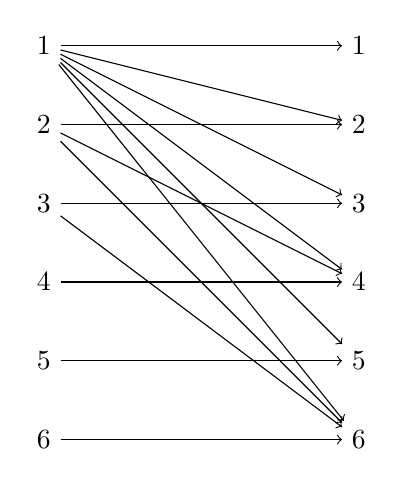
\begin{tikzpicture}
                \node (A1) at (0, 0) {1};
                \node (A2) at (0, -1) {2};
                \node (A3) at (0, -2) {3};
                \node (A4) at (0, -3) {4};
                \node (A5) at (0, -4) {5};
                \node (A6) at (0, -5) {6};

                \node (B1) at (4, 0) {1};
                \node (B2) at (4, -1) {2};
                \node (B3) at (4, -2) {3};
                \node (B4) at (4, -3) {4};
                \node (B5) at (4, -4) {5};
                \node (B6) at (4, -5) {6};

                \draw[->] (A1) -- (B1);
                \draw[->] (A1) -- (B2);
                \draw[->] (A1) -- (B3);
                \draw[->] (A1) -- (B4);
                \draw[->] (A1) -- (B5);
                \draw[->] (A1) -- (B6);

                \draw[->] (A2) -- (B2);
                \draw[->] (A2) -- (B4);
                \draw[->] (A2) -- (B6);

                \draw[->] (A3) -- (B3);
                \draw[->] (A3) -- (B6);

                \draw[->] (A4) -- (B4);

                \draw[->] (A5) -- (B5);

                \draw[->] (A6) -- (B6);
            \end{tikzpicture}
            \caption{Arrow diagram for the relation $R$ where $m$ divides $n$.}
            \label{fig:relation}
        \end{figure}
     \item \textbf{Binary matrix: } $R$ is represented by a matrix $M$ of dimensions $n \times n$ where $n = |A| = |B|$.
        \begin{figure}[h]
            \centering
            \begin{tabular}{c|cccccc}
            & 1 & 2 & 3 & 4 & 5 & 6 \\
            \hline
            1 & 1 & 1 & 1 & 1 & 1 & 1 \\
            2 & 0 & 1 & 0 & 1 & 0 & 1 \\
            3 & 0 & 0 & 1 & 0 & 0 & 1 \\
            4 & 0 & 0 & 0 & 1 & 0 & 1 \\
            5 & 0 & 0 & 0 & 0 & 1 & 0 \\
            6 & 0 & 0 & 0 & 0 & 0 & 1 \\
            \end{tabular}
            \caption{Binary matrix representation of the relation $R$ where $m$ divides $n$.}
            \label{fig:matrix}
        \end{figure}
    \item \textbf{Directed multigraph: } $R$ is represented by a directed multigraph where the vertices are elements of $A$ and $B$.
        \begin{figure}[h]
            \centering
            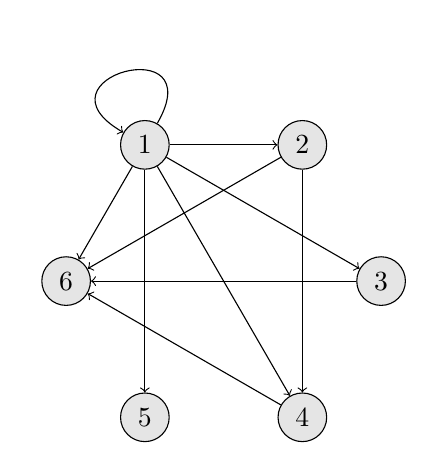
\begin{tikzpicture}
            % Nodes
            \node[circle, draw, fill=gray!20, minimum size=0.6cm] (A1) at (-1, 1.73) {1};
            \node[circle, draw, fill=gray!20, minimum size=0.6cm] (A2) at (1, 1.73) {2};
            \node[circle, draw, fill=gray!20, minimum size=0.6cm] (A3) at (2, 0) {3};
            \node[circle, draw, fill=gray!20, minimum size=0.6cm] (A4) at (1, -1.73) {4};
            \node[circle, draw, fill=gray!20, minimum size=0.6cm] (A5) at (-1, -1.73) {5};
            \node[circle, draw, fill=gray!20, minimum size=0.6cm] (A6) at (-2, 0) {6};

            % Arrows
            \draw[->, out=60, in=150, looseness=8] (A1) to (A1);
            \draw[->] (A1) -- (A2);
            \draw[->] (A1) -- (A3);
            \draw[->] (A1) -- (A4);
            \draw[->] (A1) -- (A5);
            \draw[->] (A1) -- (A6);

            \draw[->] (A2) -- (A4);
            \draw[->] (A2) -- (A6);

            \draw[->] (A3) -- (A6);

            \draw[->] (A4) -- (A6);
            \end{tikzpicture}
            \caption{Directed multigraph for the relation $R$ where $m$ divides $n$.}
            \label{fig:multigraph}
        \end{figure}
\end{enumerate}

\subsection{Domain and range of correspondences}
Let $R$ be a correspondence between $A$ and $B$, then:
\begin{enumerate}
    \item The \textbf{domain} of $R$ is the set of all elements of $A$ that are related to some element of $B$.
        \[ dom(R) = \{a \in A \mid (a,b) \in R \text{ for some } b \in B\} \subseteq A\]
    \item The \textbf{range} of $R$ is the set of all elements of $B$ that are related to some element of $A$.
        \[ ran(R) = \{b \in B \mid (a,b) \in R \text{ for some } a \in A\} \subseteq B\]
\end{enumerate}

\subsection*{Example:}
\[
A := \{1, 2, 3, 4, 5, 6\}, \quad mRn \Longleftrightarrow 2 \text{ divides } (m - n) 
\]
\[
m - n = 2k, \quad k \in \mathbb{Z} \rightarrow m = n (mod 2)
\]

\[
(1,1), (1,3), (1,5), (2,2), (2,4), (2,6), (3,1), (3,3), (3,5), 
\]
\[
(4,2), (4,4), (4,6), (5,1), (5,3), (5,5), (6,2), (6,4), (6,6)
\]

\subsection{Special relations}
\begin{enumerate}
    \item \textbf{Identity relation:} $I \subseteq A \times A$
        \[
        x,y \in A, \quad xIy \Longleftrightarrow x = y
        \]
    \item \textbf{Universal correspondence:} $U = A \times B$
    \item \textbf{Inverse correspondence:} If there exists $R \subseteq A \times B$, then: $R^{-1} \subseteq B \times A$
        \[
        R := \{(b,a) \in B \times A \mid (a,b) \in R\}
        \]
\end{enumerate}

\subsection{Properties of correspondences}
\begin{enumerate}
    \item \textbf{Reflexivity:} $R \subseteq A \times A$ is reflexive if and only if $(a,a) \in R$ for all $a \in A$.
    \item \textbf{Symmetry:} $R \subseteq A \times A$ is symmetric if and only if $(a,b) \in R \Leftrightarrow (b,a) \in R$.
    \item \textbf{Antisymmetry:} $R \subseteq A \times A$ is antisymmetric if and only if whenever \\ 
    $(a,b) \in R$ and $(b,a) \in R \implies a = b$.
    \item \textbf{Transitivity:} $R \subseteq A \times A$ is transitive if and only if whenever \\
    $(a,b) \in R$ and $(b,c) \in R \implies (a,c) \in R$.
\end{enumerate}

\subsection*{Example:}
\[
A := \{a, b, c, d\}, \quad R := \{(a,a), (a,b), (a,c), (b,a), (b,b), (b,c), (b,d), (d,d)\}
\]
\begin{enumerate}
    \item Reflexive: $(c,c) \notin R \implies R$ is not reflexive.
    \item Symmetric: $(a,c) \in R$, but $(c,a) \notin R \implies R$ is not symmetric.
    \item Antisymmetric: $(a,b) \in R, (b,a) \in R$, but $a \neq b \implies R$ is not antisymmetric.
    \item Transitive: $(a,b) \in R, (b,d) \in R$, but $(a,d) \notin R \implies R$ is not transitive.
\end{enumerate}

\subsection*{Example:}
\[
A := \{1, 2, 3, 4, 5, 6\}, \quad R := \{(m,n) \mid m \text{ divides } n\}
\]
\begin{enumerate}
    \item Reflexive: $\forall m \in A \implies m \text{ divides } m \implies R$ is reflexive.
    \item Symmetric: $m \text{ divides } n \implies n \text{ does not divide } m \implies R$ is not symmetric.
    \item Antisymmetric: $m \text{ divides } n, n \text{ divides } m \implies m = n \implies R$ is antisymmetric.
    \item Transitive: $m \text{ divides } n, n \text{ divides } p \implies m \text{ divides } p \implies R$ is transitive.
\end{enumerate}

\subsection*{Example:}
\[
A = \mathbb{N} \times \mathbb{N} = \{(a,b) \mid a,b \in \mathbb{N}\}, \quad R = \{\left((a,b), (c,d)\right) \mid a + d = b + c\}
\]
\begin{enumerate}
    \item Reflexive: $(a,b) + (b,a) = 2b = 2a \implies R$ is reflexive.
    \item Symmetric: $(a,b) + (c,d) = (c,d) + (a,b) \implies R$ is symmetric.
    \item Antisymmetric: $(a,b) + (c,d) = (c,d) + (a,b) \nRightarrow (a,b) = (c,d) \implies R$ is not antisymmetric.
    \item Transitive: $(a,b) + (c,d) = (c,d) + (e,f) \implies R$ is transitive.
\end{enumerate}

\subsection{Operations with correspondences}
\begin{enumerate}
    \item \textbf{Union:} $R \cup S = \{(a,b) \in A \times A \mid (a,b) \in R \text{ or } (a,b) \in S\}$
    \item \textbf{Intersection:} $R \cap S = \{(a,b) \in A \times A \mid (a,b) \in R \text{ and } (a,b) \in S\}$
\end{enumerate}

Both Union and Intersection preserve reflexivity and symmetry:
\begin{enumerate}
    \item If $R$ and $S$ are reflexive, then 
    \[
    \forall a \in A \quad (a,a) \in R \text{ and } (a,a) \in S \implies (a,a) \in R \cup S \text{ and } (a,a) \in R \cap S
    \]
    \item $R$ and $S$ are symmetric
    \[
    \text{If } (a,b) \in R \implies (b,a) \in R \text{ and } (c,d) \in S \implies (d,c) \in S 
    \]
\end{enumerate}

However, only Intersection preserves antisymmetry and transitivity.

\subsubsection{Counterexamples for the union}
\begin{enumerate}
    \item \textbf{Antisymmetry:} $R = \{(a,b)\}$ and $S = \{(b,a)\} \implies \text{antisymmetric, but }\\
    R \cup S = \{(a,b), (b,a)\} \text{ is not antisymmetric}$
    \item \textbf{Transitivity:} $R = \{(a,b)\}$ and $S = \{(b,c)\} \implies \text{transitive, but }\\
    R \cup S = \{(a,b), (b,c)\} \text{ is not transitive}$
\end{enumerate}

\subsection{Types of relations}
\begin{enumerate}
    \item \textbf{Equivalence relation:} A set $R \subseteq A \times A$ is an equivalence relation if and only if it is reflexive, symmetric, and transitive.
    \item \textbf{Order relation:} A set $R \subseteq A \times A$ is an order relation if and only if it is reflexive, antisymmetric, and transitive.
\end{enumerate}

\subsubsection{Equivalence relations}
\subsection*{Example:}
\[
A := \{\text{people living in Spain}\}, \quad R := \{(x,y) \mid x \text{ and } y \text{ live in the same municipality}\}
\]
\begin{enumerate}
    \item Reflexive: $x$ lives in the same municipality as $x$.
    \item Symmetric: If $x$ lives in the same municipality as $y$, then $y$ lives in the same municipality
    \item Transitive: If $x$ lives in the same municipality as $y$ and $y$ lives in the same municipality as $z$, then $x$ lives in the same municipality as $z$.
\end{enumerate}

\subsection*{Example:}
\[
A := \mathbb{R}^2 - \{(0,0)\}, \quad R := \{(x,y) \mid x \text{ and } y \text{ are on the same line through the origin}\}
\]
\begin{enumerate}
    \item Reflexive: $(0,0)$ is on the same line through the origin as $(0,0)$.
    \item Symmetric: If $x$ is on the same line through the origin as $y$, then $y$ is on the same line through the origin as $x$.
    \item Transitive: If $x$ is on the same line through the origin as $y$ and $y$ is on the same line through the origin as $z$, then $x$ is on the same line through the origin as $z$.
\end{enumerate}

\subsubsection{Equivalence class}
Let $A, \quad R \subset A \times A$ be an equivalence relation, then the class of equivalence of $x \in A$ is defined as 
\[
[x] = \{y \in A \mid (x,y) \in R\}
\]

The set of classes of equivalence of $R$ is a covering of $A$
\[
A = \bigcup_{x \in A}[x], \quad \text{remember } x \in [x] \text{ because of reflexivity and also } xRx \quad \forall x \in A
\]

Furthermore, $\bigcup_{x \in A}[x]$ is a partition of $A$

\paragraph{Theorem:} Let $A$ be a set, $R$ an equivalence,
\[
xRy \Longleftrightarrow [x] = [y]
\]

\paragraph{Proof:} $[x] = [y]$ \\
We need to prove:
\[
\begin{cases}
    [x] \subseteq [y] \\
    [y] \subseteq [x]
\end{cases}
\]
\[
\text{where } [x] = \{z \in A \mid xRz\}, \quad [y] = \{z \in A \mid yRz\}
\]

$[x] \subseteq [y]$: \\
Let $z \in [x]$, then $xRz \implies xRy \implies yRz \implies z \in [y]$.

Let $z \in [y]$, then $yRz \implies yRx \implies xRz \implies z \in [x]$.

The classes of equivalence form a partition of $A$.
\[
\forall x \in A, \quad x \in [x]
\]

If $[x]$ and $[y]$ have a common element, $z \in [x] \cap [y]$, then $[x] = [y]$.

\subsection{Quotient set}
Let $A$ be a set, $R$ an equivalence relation on $A$, then the quotient set of $A$ by $R$ is defined as:
\[
A/R = \{[x] \mid x \in A\}
\]

which means that $A/R$ is the set of all classes of equivalence of $A$ with respect to $R$.

\subsection*{Example:}
\[
A = \{a, b, c, d, e \}
\]
\[
R = \{(a,a), (b,b), (c,c), (d,d), (e,e), (a,b), (b,a), (a,c), (c,a), (b,c), (c,b)\}
\]

\[
A/R = \{\{a,b,c\}, \{d\}, \{e\} \}, \quad \text{where } [a] = [b] = [c]
\]

\begin{figure}[h]
    \centering
    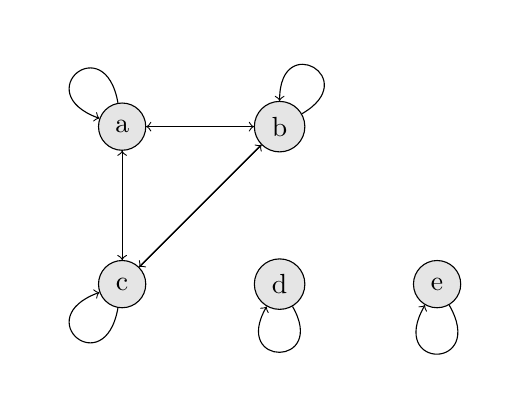
\begin{tikzpicture}
        % Nodes
        \node[circle, draw, fill=gray!20, minimum size=0.6cm] (A) at (0, 0) {a};
        \node[circle, draw, fill=gray!20, minimum size=0.6cm] (B) at (2, 0) {b};
        \node[circle, draw, fill=gray!20, minimum size=0.6cm] (C) at (0, -2) {c};
        \node[circle, draw, fill=gray!20, minimum size=0.6cm] (D) at (2, -2) {d};
        \node[circle, draw, fill=gray!20, minimum size=0.6cm] (E) at (4, -2) {e};

        % Arrows
        \draw[->, in = 160, out = 100, looseness = 8] (A) to (A);
        \draw[->, in = 90, out = 30, looseness = 7] (B) to (B);
        \draw[->, in = 200, out = 260, looseness = 8] (C) to (C);
        \draw[->, in = 240, out = 300, looseness = 7] (D) to (D);
        \draw[->, in = 240, out = 300, looseness = 8] (E) to (E);
        \draw[->] (A) -- (B);
        \draw[->] (A) -- (C);
        \draw[->] (B) -- (C);
        \draw[->] (C) -- (B);
        \draw[->] (B) -- (A);
        \draw[->] (C) -- (A);

    \end{tikzpicture}
    \caption{Directed multigraph for the relation $R$ where $a$, $b$, and $c$ are related to each other, and $d$, and $e$ are related to themselves.}
    \label{fig:multigraph2}
\end{figure}

\subsubsection{Example: Modular arithmetic}
\[
a, b \in \mathbb{Z}, \quad a \equiv b \mod n \Longleftrightarrow a - b = kn, \quad k \in \mathbb{Z}, \quad n \in \mathbb{N}
\]

\[
aRb \Longleftrightarrow a \equiv b \mod n \text{ is an equivalence relation}
\]

\[
\textbf{Reflexive: } a = a + 0n \implies a \equiv a \mod n \implies aRa
\]

\[
\textbf{Symmetric: } a \equiv b \mod n \implies a - b = kn 
\]
\[
\implies b - a = (-k)n \implies b \equiv a \mod n \implies aRb \implies bRa
\]

\[
\textbf{Transitive: } \begin{cases}
    a - b = kn \\
    b - c = ln
\end{cases} \implies a - c = (k + l)n \implies a \equiv c \mod n \implies aRc
\]

 \subsubsection{Equivalence classes: quotient set of $\mathbb{Z}$ by $n\mathbb{Z}$}
\[
[0] = \{x \in \mathbb{Z} \mid 0 - x = kn, \quad k \in \mathbb{Z}\} = \{x \in \mathbb{Z} \mid x = kn, \quad k \in \mathbb{Z}\}
\]

For $n \geq 2$:
\[
[1] = \{x \in \mathbb{Z} \mid 1 - x = kn, \quad k \in \mathbb{Z}\} = \{x \in \mathbb{Z} \mid 1 - x = kn, \quad k \in \mathbb{Z}\}
\]
\[ \vdots \]
\[
[n] = \{x \in \mathbb{Z} \mid n - x = kn, \quad k \in \mathbb{Z}\} = \{x \in \mathbb{Z} \mid x = kn, \quad k \in \mathbb{Z}\}
\]

\[
\mathbb{Z}/n\mathbb{Z} = \{[0], [1], \ldots, [n-1]\}
\]
\[
xy = (a + kn)(b + ln) = ab + (al + bk + kln)n
\]

In modular arithmetic: 
\[
[a] + [b] = [a + b], \quad [a] \cdot [b] = [a \cdot b]
\]

\[
x \in [a], \quad y \in [b] \implies x = a + kn, \quad y = b + ln
\]
\[
x + y = a + b + (k + l)n \implies x + y \in [a + b]
\]

\subsection{Order relations}
Let $A$ be a set, $R \subseteq A \times A$ an order relation. If $R$ is reflexive, antisymmetric, and transitive, then $R$ is an order relation.

\subsection*{Example:}
\[
R, \quad xRy \Longleftrightarrow x \leq y
\]

\begin{enumerate}
    \item Reflexive: $x \leq x$
    \item Antisymmetric: $x \leq y, y \leq x \implies x = y$
    \item Transitive: $x \leq y, y \leq z \implies x \leq z$
\end{enumerate}

\subsection*{Example:}
Let $A$ be a set, $P(A)$ the set of all subsets of $A$.
\[
B, C \in P(A), \quad B \subseteq C \Longleftrightarrow B \leq C
\]

\begin{enumerate}
    \item Reflexive: $B \subseteq B$
    \item Antisymmetric: $B \subseteq C, C \subseteq B \implies B = C$
    \item Transitive: $B \subseteq C, C \subseteq D \implies B \subseteq D$
\end{enumerate}

\subsection*{Example:}
\[
A = \{a,b,c\}, \quad P(A) = \{\emptyset, \{a\}, \{b\}, \{c\}, \{a,b\}, \{a,c\}, \{b,c\}, \{a,b,c\}\}
\]
\[
B, C \in P(A), \quad B \subseteq C \Longleftrightarrow B \leq C
\]
\[
\{a\} \leq \{a,b\}, \quad \text{but } \{a\} \nleq \{b,c\}
\]

\subsection{Theorem:}
Let $A$ be a set, with $\leq$ an order relation on $A$. Then:
\[
B \subseteq A \implies B \text{ is also an ordered set }
\]

\begin{enumerate}
    \item \textbf{Reflexive:} $x \in B \implies x \leq x$
    \item \textbf{Antisymmetric:} $x \leq y, y \leq x \implies x = y$
\end{enumerate}

\subsection{Notable elements in an order}
Let $A$ be a set, $\leq$ an order relation on $A$ and $B \subseteq A$. Then:
\begin{enumerate}
    \item $x \in A$ is an \textbf{upper bound} of $B$ if:
    \[
    \forall y \in B \implies y \leq x, \quad \text{(B is bounded from above)}
    \]
    \item $x \in A$ is a \textbf{lower bound} of $B$ if:
    \[
    \forall y \in B \implies x \leq y, \quad \text{(B is bounded from below)}
    \]
    Note: if $B$ is bounded from above and below, then $B$ is bounded.
    \item $x \in A$ is the \textbf{supremum} of $B$ if:
    \[
    x \leq y, \quad \forall y \in B, \quad \text{where } y \text{ is any upper bound of } B
    \]
    In case $x \in B$, then $x$ is the maximum of $B$.
    \item $x \in A$ is the \textbf{infimum} of $B$ if:
    \[
    y \leq x, \quad \forall y \in B, \quad \text{where } y \text{ is any lower bound of } B
    \]
    In case $x \in B$, then $x$ is the minimum of $B$.
    \item $y \in B$ is a \textbf{maximal element} of $B$ if:
    \[
    \nexists x \in B \text{ such that } y \leq x
    \]
    \item $y \in B$ is a \textbf{minimal element} of $B$ if:
    \[
    \nexists x \in B \text{ such that } y \geq x
    \]
\end{enumerate}

\paragraph{Theorem: } The supremum and infimum of a set are unique.
Let $\gamma, \gamma'$ be suprema of $B$, then:
\[
\gamma \leq \gamma' \text{ and } \gamma' \leq \gamma \implies \gamma = \gamma'
\]

\subsection*{Example:}
\[
A = \{a,b,c\}, \quad W = P(A) - A = \{\emptyset, \{a\}, \{b\}, \{c\}, \{a,b\}, \{a,c\}, \{b,c\}\}
\]
\[
W \subseteq P(A), \quad \emptyset \subset w \in W \implies \emptyset \leq w \quad \forall w \in W
\]
\[
\implies \emptyset \text{ is a lower bound of } W, \quad \emptyset \text{ is the infimum of } W, \quad \emptyset \text{ is the minimum of } W
\]

Also, $A$ is an upper bound of $W$, $A$ is the supremum of $W$, but $A$ is not the maximum of $W$.

The empty set is also a minimal element of $W$. However, there are three maximal elements in $W$: $\{a,b\}, \{a,c\}, \{b,c\}$. (Note that $A$ contains the but $A \notin W$).

\subsection*{Example:}
\[
A = \mathbb{N}, m \leq n \text{ if } m \text{ divides } n, \quad B = \{2,3,4,5,6,7,8\}
\]
\[
\text{The minimals of $B$ are } 2, 3, 5, 7, \text{ and the maximals are } 5,6,7,8
\]

Observe that 5 and 7 are both maximal and minimal elements of $B$.
\[
\text{The supremum of $B$ is the m.c.m. of all elements of $B$} = 2^3 \cdot 3 \cdot 5 \cdot 7 = 840, 
\]
\[
\text{and the infimum is the l.c.d. of all elements of $B$} = 1
\]

\subsection{Total order}
Let $A$ be a set, $\leq$ an order relation on $A$. $\leq$ is a total order if and only if:
\[
\forall x, y \in A \quad x \leq y \text{ or } y \leq x
\]

\subsection*{Examples:}
The usual order of $\mathbb{N}$ is a total order.

The alphabetical order of words is a total order.




\end{document}